\chapter{Approach}\label{chap:approach}
In this section, we provide a layout of our approach to find similar tools. It includes procedures to extract and clean tools data, learn vectors for each tool, find similarity (correlation) matrices and optimize the combination of these matrices to estimate a final similarity matrix (figure 4). 
\section{Extract tools data}    
As Galaxy is an open-source project, the repositories of tools are stored at GitHub\footnote{One example:\url{https://github.com/galaxyproject/tools-iuc/tree/master/tools}}. In these tool repositories, the xml files which start a "tool" tag belong to a tool. We read all of these xml files, extract information from a few of the tool attributes and collect them in a tabular file. This tabular file contains the information about all the tools.

\begin{figure}[h]
\begin{centering}
    {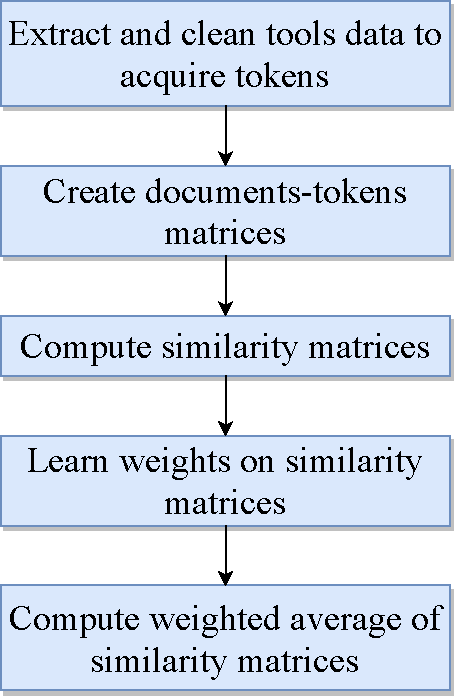
\includegraphics[scale=0.7]{figures/tool_sim_flow.pdf}}
    \caption[Sequence of steps to find similar tools]{\textbf{Sequence of steps to find similar tools}: The flowchart shows a series of steps used to establish similarity among tools using approaches from natural language processing to compute text similarity scores and optimization to combine optimally.}
\end{centering}
\end{figure}
    
\subsection{Select tools attributes}
A tool has multiple attributes like input and output file types, help text, name, description, citations and more. But all of these attributes are not important and do not generally identify a tool exclusively. To collect distinguishing information about a tool, we consider only these attributes:
\begin{itemize}
	\item Input and output file types
	\item Name and description
	\item Help text
\end{itemize}
Moreover, we combine the input and output file types and name and description respectively as they are of similar nature. These combined attributes give complete information about a tool's file types (input and output types) and its functionality (name and description). Further, we take help text attribute as well which is larger in size compared to the previous two. It can also be empty for some tools. Apart from being large in size, it is noisy. It provides more information about the usage of a tool. Generally in the first few lines, it gives a detailed explanation of a tool's functions. Further, it explains how the input data should be supplied to a tool or how an input data looks like. Much of the information contained by this attribute is not important to clearly distinguish a tool. Hence, we decide to use only the first few lines ($4$ lines) of text present in help text attribute of a tool which illustrates its core functionality. The rest of the information in help text is discarded. The decision to select only the first $4$ lines is empirical.

\subsection{Clean tools data}
\subsubsection{Remove duplicates and stopwords}
    The collected data for tools is raw as it contains lots of commonplace and duplicate items which do not add value. These items should be removed to get $tokens$ which are unique and useful. For example, a tool "bamleftalign" has input files as "bam" and "fasta" and output file as "bam". While combining these file types, we discard the repeated ones. In this case, we consider the file types as "bam" and "fasta". The other attributes we deal with are different from the file types. The files types are already in the form of $tokens$. But, in the attributes like name and description and help text, the words come from English and the explanation contains complete or partially complete sentences. Hence, to process this information, we need strategies that are prevalent in natural language processing\footnote{\url{https://www.ncbi.nlm.nih.gov/pmc/articles/PMC3168328/}}. The sentences we write in English contain many words and has different parts. These parts include subject, object, preposition, interjection, verbs, adjectives, adverbs, articles and many others. For our processing, we need only those tokens (words) which categorize a tool uniquely and do away with multiple parts of speech present in the sentences. For example, a tool named $tophat$ has a name and description as "TopHat for Illumina Find splice junctions using RNA-seq data". The words like "for", "using" and "data" do not give much value as they can be present for many other tools. These words are called as "stopwords"\footnote{\url{https://www.ranks.nl/stopwords}} and we selectively discard them. In addition, we remove numbers and convert all the tokens to lower case.
 
\subsubsection{Use stemming}
After removing duplicates and stopwords, our data is clean and contain tokens which uniquely identify corresponding tools. When we frame sentences, we follow grammar which constrains us to use different forms of the same word in varying contexts. For example, a word "regress" can be used in multiple forms as "regresses" or "regression" or "regressed". They share the same root and point towards the same concept. If many tools use this word in varying forms, it is beneficial to converge all the different forms of a word to one basic form. This process is called stemming\footnote{\url{https://nlp.stanford.edu/IR-book/html/htmledition/stemming-and-lemmatization-1.html}}. We use NLTK\footnote{\url{http://www.nltk.org/}} package for stemming. It enables us to reduce the size to tokens while keeping the meaning of these tokens same across all the tools.

\begin{figure}[h]
\begin{centering}
    {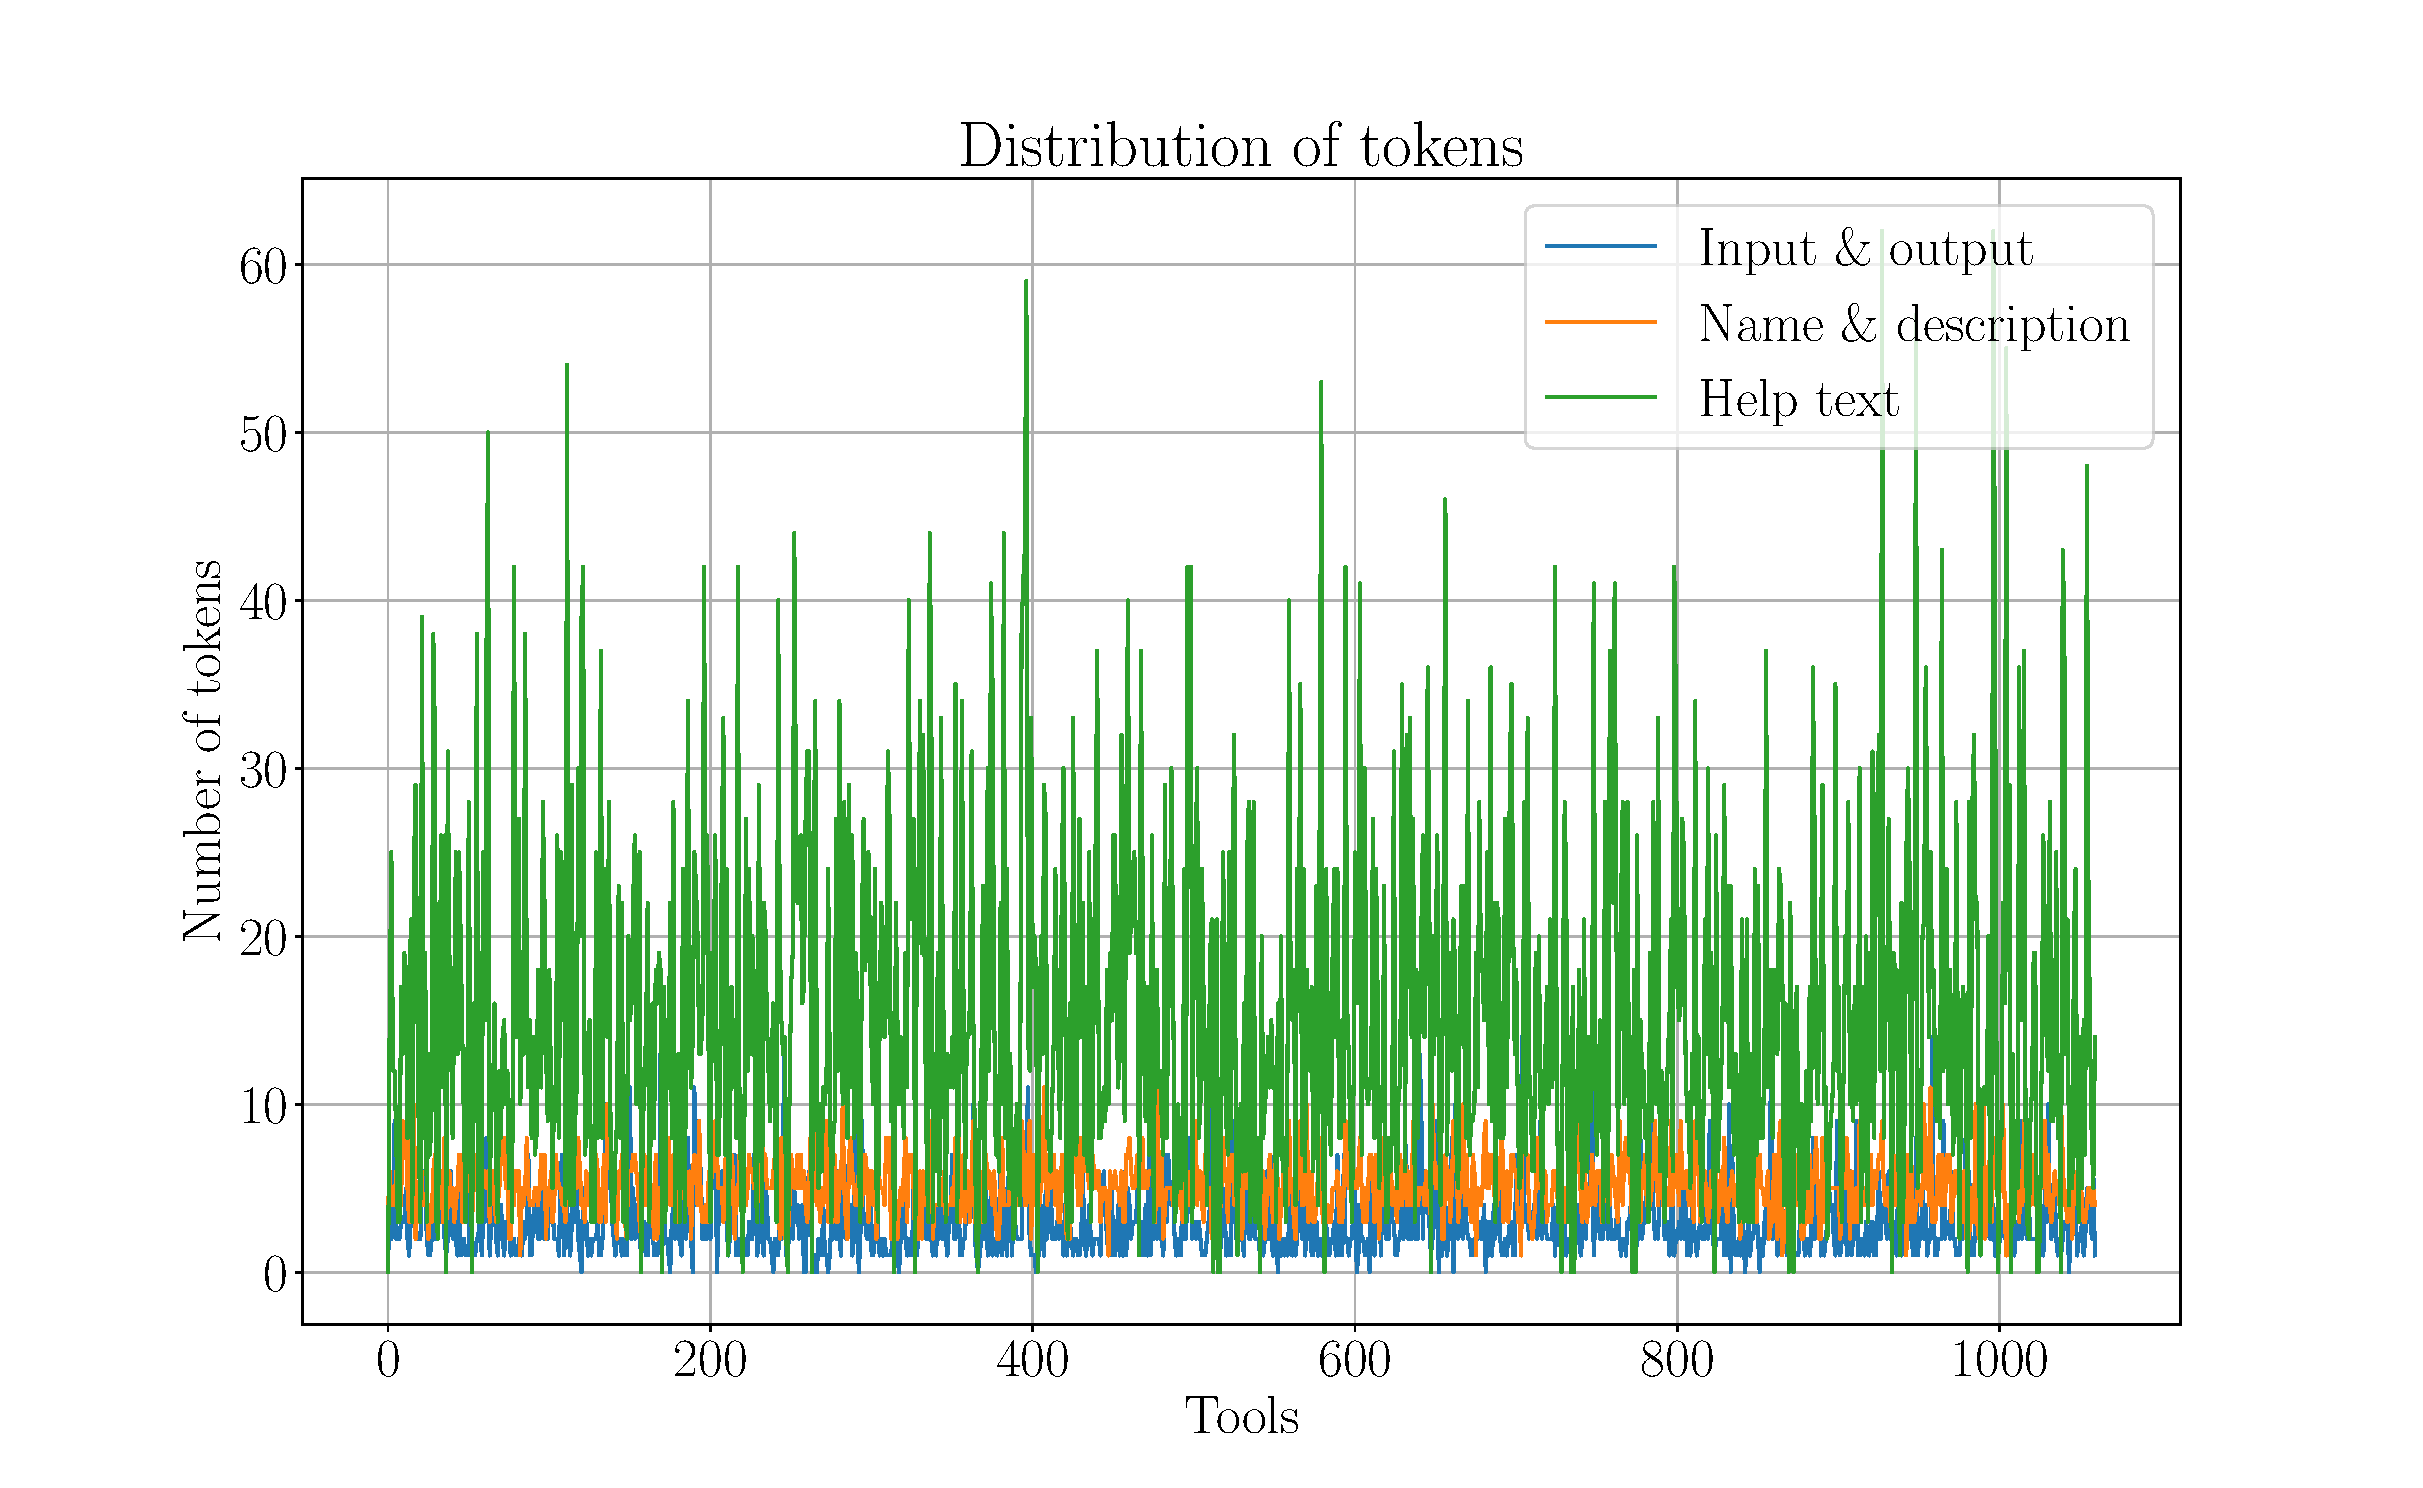
\includegraphics[scale=0.4]{figures/Tokens_dist.pdf}}
    \caption[Distribution of tokens for all the attributes of tools]{\textbf{Distribution of tokens (words) for all the attributes of tools}: The plot shows a distribution of tokens for input and output file types, name and description and help text attributes of tools. The help text attribute contains more number of tokens compared to the other two. The input and output file types attribute contains a lower number of tokens compared to the other two attributes. }
\end{centering}
\end{figure}

\begin{figure}[h]
\begin{centering}
    {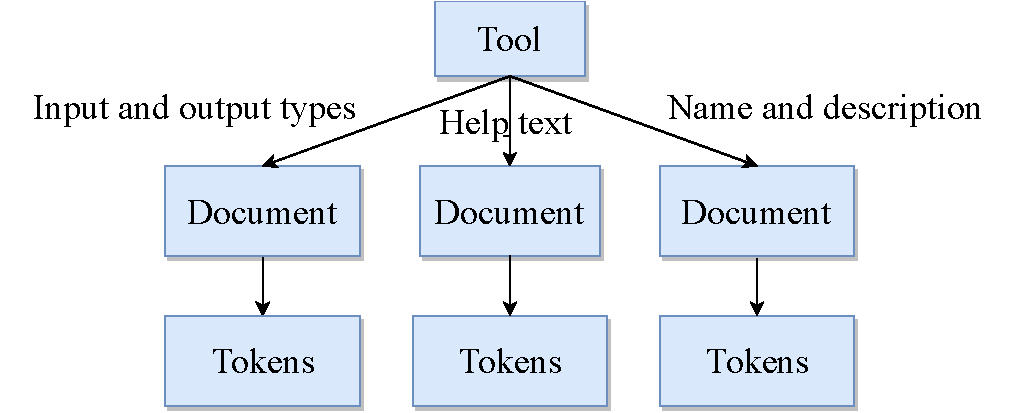
\includegraphics[scale=0.7]{figures/tool-document-tokens.pdf}}
    \caption[Tool, document and tokens]{\textbf{Relationship between a tool, its documents and their tokens}: The image shows that a tool has three documents corresponding to each attribute and each document contains tokens. For all the tools, we have documents equal to the number of tools for each attribute. The number of tokens in each document varies. Minimum number of tokens for any document can be 0.}
\end{centering}
\end{figure}

\subsubsection{Learn relevance for words}
From now on, we use a term "token" for each word. For example, a tool's name contains "regress, perform" as a set of tokens (words). After discarding duplicate tokens, stopwords and using stemmed words, we have a set of meaningful tokens for all the three attributes - input and output file types, name and description and help text. We call these sets as "documents" (figure 6). The tokens present in these documents do not carry equal importance. Some tokens are more relevant to a document and some not so relevant. We need to find out importance factors for all tokens in a document. Using these factors, we can arrange them in big, sparse documents-tokens matrix. In these matrices, each row represents a document and each column belongs to one token. To compute these importance factors, we use BM25 (bestmatch25) \cite{Robertson:2009:PRF:1704809.1704810}. Let's associate some variables to be used in explaining this algorithm.

\begin{itemize}
	\item Token frequency\footnote{\url{https://nlp.stanford.edu/IR-book/pdf/06vect.pdf}} ($tf$)
	\item Inverted document frequency ($idf$)
	\item Average document length ($|D|_{avg}$)
	\item Number of documents ($N$)
	\item Size of a document ($|D|$)
\end{itemize}
    
Token frequency ($tf$) specifies the count of a token's occurrence in a document. If a token "regress" appears twice in a document, its $tf$ is $2$. This can also be understood as a weight given to this term. Inverted document frequency for a token is defined as:

\begin{equation}
idf = \log \frac{N}{df}
\end{equation}
 
where $df$ is the count of the documents in which this token is present and $N$ is the total number of documents. If we randomly sample a document, then the probability of this token to be present in this document is $ p_i = \frac{df}{N} $. From information theory, we can say that the information contained by this event is $ - \log p_i $. The entity $idf$ is higher when a token appears in a lesser number of documents. It means that this token is a good candidate for representing that document and thereby, possesses a higher power to distinguish between documents. The tokens which appear in many documents are not good representatives as they tend to be commonplace. Average document length ($|D|_{avg}$) is the average number tokens for all the documents. Size of a document ($|D|$) is the count of all the tokens for that document. 

\begin{equation}
\alpha = (1-b) + \frac{b \cdot |D|}{|D|_{avg}}
\end{equation}

\begin{equation}
tf^* = tf \cdot \frac{k+1}{k \cdot \alpha + tf}
\end{equation}

\begin{equation}
BM25_{score} =tf^* \cdot idf
\end{equation}

where $k$ and $b$ are hyperparameters. Using the equation $4$, we compute the relevance score for each token in all the documents. Table 1 shows scores for a few documents where the tokens are present with their respective BM25 scores. In this way, we arrange document-tokens matrix for all the attributes of tools. For input and output file types, these matrix entries will have only two value, $1$ if a token is present for a document and $0$ if not. For other attributes, relevance scores are positive real numbers. This method of representing documents with their tokens is called vector space model as each document represents a vector of tokens.

\begin{table}[ht]
\begin{center}
    \begin{tabular}{|l|l|l|l|l|l|}
        \hline
        Documents/tokens   & regress & linear & gap & mapper & perform \\ \hline
        LinearRegression   & 5.22 & 4.1 & 0.0 & 0.0  & 3.84 \\ \hline
        LogisticRegression & 3.54 & 0.0 & 0.0 & 0.0  & 2.61 \\ \hline
        Tophat2            & 0.0  & 0.0 & 1.2 & 1.47 & 0.0 \\ \hline
        Hisat              & 0.0  & 0.0 & 0.0 & 0.0  & 0.0 \\ \hline
    \end{tabular}
    \end{center}
    \caption[A sparse documents-tokens matrix]{\textbf{A sparse documents-tokens matrix}: This table shows a matrix of tools (documents) arranged along the rows and tokens along the columns. Each value in the matrix is a weight (relevance-factor) assigned to a token for a document. This matrix is sparse containing mostly zeros as the number of tokens is significantly large compared to the number of tokens present in a document. This table shows a sample of how actual documents-tokens matrix would look like.}
    \label{tab:accuracy}
\end{table}

Figure 7 shows a heatmap for documents-tokens matrices that belong to name and description and help text attributes. We can see that these plots are sparse. Each entry in these matrices contains BM25 score for each token in a document. This representation tells us which tokens are better representatives and which are not. But, they do not tell us anything about the co-occurrence of tokens in a document. It tells us that a token is important for a document if the BM25 score is higher but it does not tell us anything about its relation to other tokens. Due to this limitation, it does not acknowledge the presence of "concepts" or "context" hidden in a document. A concept in a document can be realised when we see the relation among a few words. To illustrate this idea, let's take an example of three words - "New York City". These three words mean little or point to different things if we look at them separately. But, if we see them together, it points towards a concept. The BM25 model lacks the ability to find the correlation among tokens. To learn the hidden concepts within documents and find correlation among multiple tokens, we explore two ideas:
\begin{itemize}
\item Latent Semantic Indexing/Analysis\footnote{\url{http://lsa.colorado.edu/papers/dp1.LSAintro.pdf}}
\item Paragraph Vectors
\end{itemize}

Using these approaches, we learn dense, multi-dimensional vector for each document instead of sparse vectors. 

\begin{figure}[h]
\begin{centering}
    {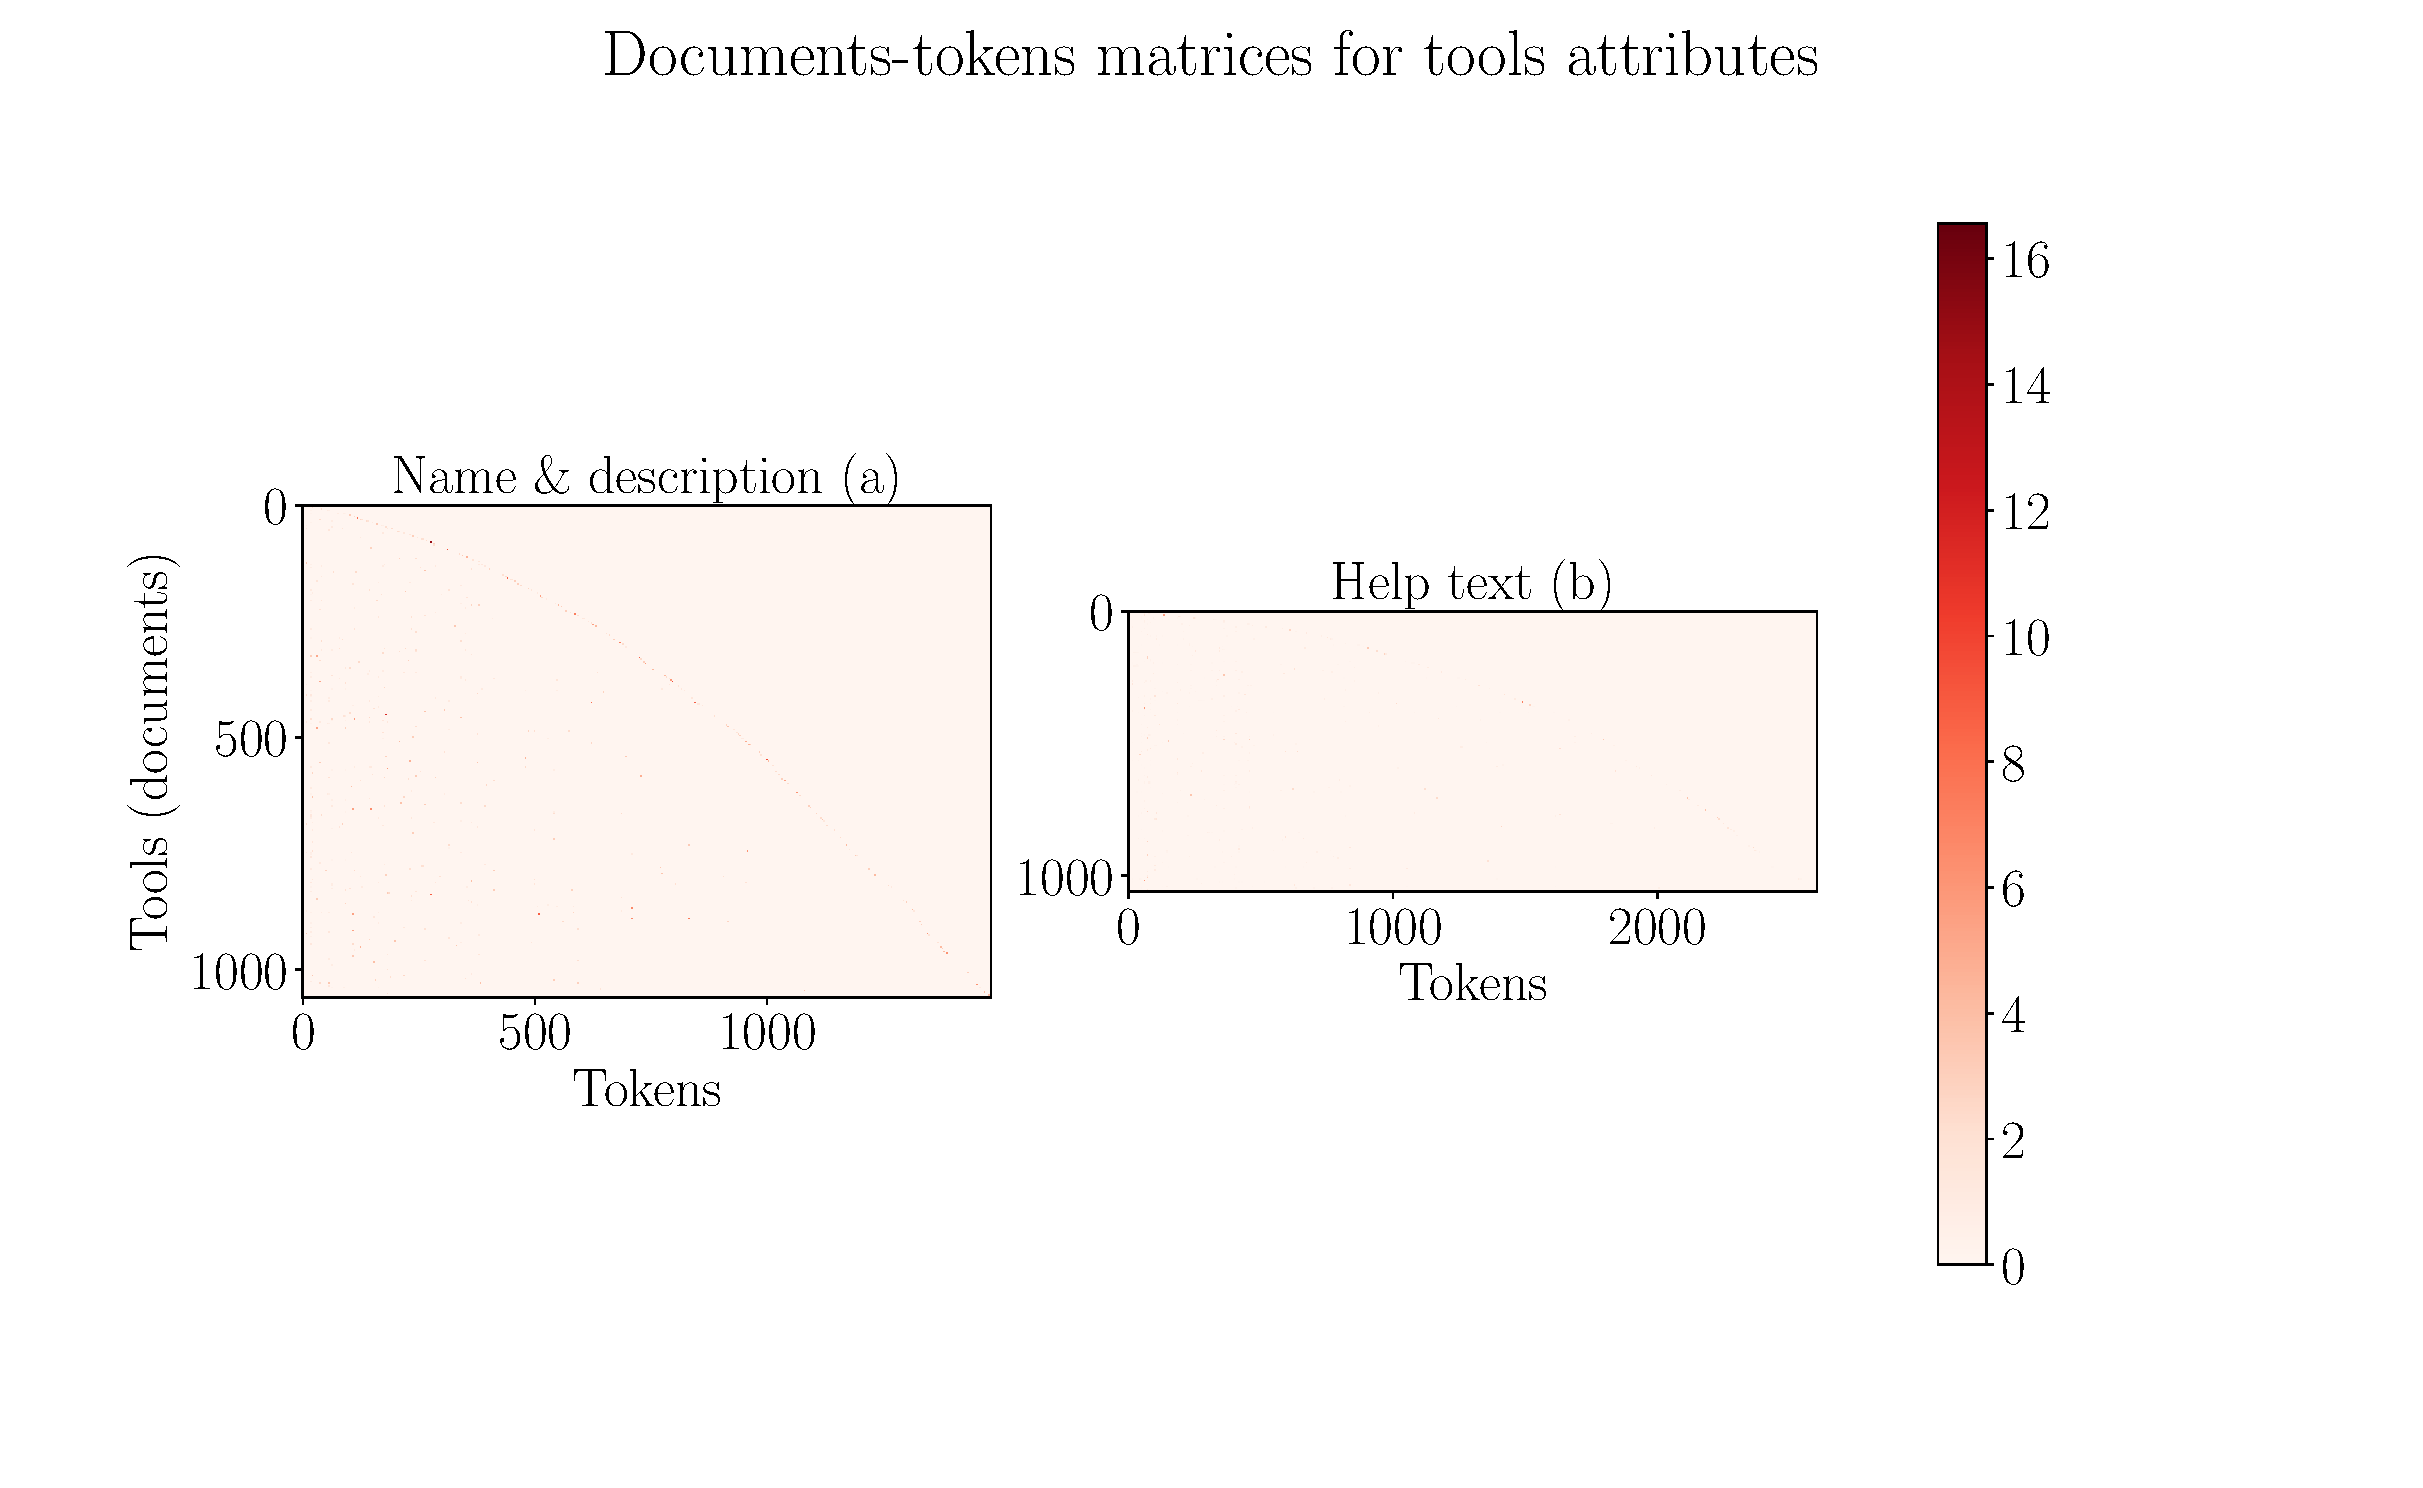
\includegraphics[scale=0.4]{figures/Document_tokens_full_rank.pdf}}
    \caption[Heatmap for documents-tokens matrices]{\textbf{Heatmap for documents-tokens matrices}: The plot shows a heatmap of documents-tokens matrices for name and description and help text attributes. We see that the matrices are sparse containing only few darker spots. The help text matrix is more sparse than name and description matrix as the former contains more number of tokens. We exclude the documents-tokens matrix of input and output file types because we do not intend to find concepts among file types. For the other two matrices, we estimate their dense, lower-rank approximations.}
\end{centering}
\end{figure}

\section{Learn dense vector for a document}
\subsection{Latent semantic indexing}
    It is a mathematical way to learn the hidden (latent) concepts in documents by computing a low-rank representation of a documents-tokens matrix \cite{Foltz1996, Shapiro2000, Landauer1998}. This low-rank matrix is dense (figure 12). We use singular value decomposition ($SVD$) for this decomposition. The optimal rank to which a matrix needs to be decomposed to get the best approximation of the full-rank matrix is empirical in nature. We choose ranks from higher to lower for decomposition and consequently the sum of singular values also decreases with the rank. This decomposition follows the equation:
    
    \begin{equation}
    X_{n \times m} = U_{n \times n} \cdot S_{n \times m} \cdot V_{m \times m}^T
    \end{equation}
    
    where $n$ is the number of documents and $m$ is the number of tokens. $S$ is a diagonal matrix containing the singular values in descending order. It contains the weights of the concepts present in the documents-tokens matrix. The matrices $U$ and $V$ and orthogonal matrices and satisfy:
    
    \begin{equation}
    U^T \cdot U = I_{n \times n}
    \end{equation}
    \begin{equation}
    V^T \cdot V = I_{m \times m}
    \end{equation}
    
\begin{figure}[h]
\begin{centering}
    {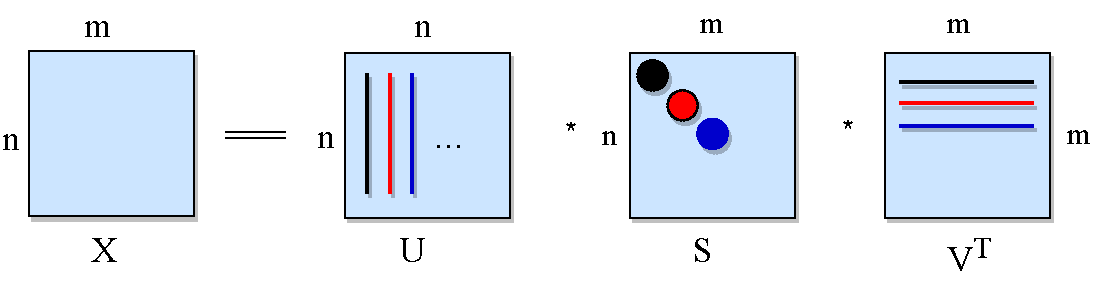
\includegraphics[scale=0.7]{figures/usv.pdf}}
    \caption[Pictorial representation of singular value decomposition]{\textbf{Singular value decomposition}: The image shows that how a matrix is decomposed using singular value decomposition. A matrix $X$ is decomposed into three matrices, $U$, $S$ and $V$. The $k$ ($<m$) most important dimensions are kept and the rest are discarded. The value of $k$ is empirical and can be estimated using optimization taking Frobenius norm as an error function.}
\end{centering}
\end{figure}

Figure 8 explains\footnote{\url{http://theory.stanford.edu/~tim/s15/l/l9.pdf}} how the $SVD$ of a matrix is carried out. The matrix $U$ contains information about how the tokens, arranged along the columns, are mapped to concepts. The matrix $V$ stores information about how the concepts are mapped to documents arranged along the rows.

\subsubsection{Low-rank approximation}
The low-rank approximation of a matrix is important to discard the features which are non-repeating. These features with low scaling factors represent noise and by discarding these unimportant features, we can collect the latent relations present in the documents-tokens matrices. We have seen that our documents-tokens matrices suffer from sparsity and exhibit no relation among tokens. The low-rank approximation deals with these issues. The resulting matrices are dense and contain top singular values (which are higher in magnitude). The singular values which are small (the last entries of the $S$ matrix along the diagonal) are discarded \cite{DBLP:journals/corr/Yang15b}. The low-rank approximation $X_k$ ($k<m$) is computed as:
    \begin{equation}
    X_{n \times m} = U_{k} \cdot S_{k} \cdot V_{k}^T
    \end{equation}
    where $U_{k}$ is the first $k$ columns of $U$, $V_{k}$ is the first $k$ rows and $S$ is the first $k$ singular values. $k$ is an empirical parameter. $X_k$ is called as the rank-k approximation of the full-rank matrix $X$. Figure 10 shows how the rank varies with the sum of singular values for documents-tokens matrices for all the attributes. Figure 11 shows how the fraction of the sum of singular values vary with the fraction of ranks of documents-tokens matrices for all the attributes. The percentage rank is $k \div K$ where $1 <= k <= K$ and $K$ is the original (full) rank of a matrix. By taking fractions, we bring all the three plots from figure 10 into one plot. From figure 11, we can say that if we reduce the ranks of matrices to $70\%$ of the full-rank, we can still capture $\approx 90\%$ of the sum of singular values. The reduction to half of the full-rank achieves $\approx 80\%$ of the sum of singular values. We show the variation for input and output file types in figure 10 and 11 but we do not reduce its rank. That is for completeness.

\begin{figure}[h]
\begin{centering}
    {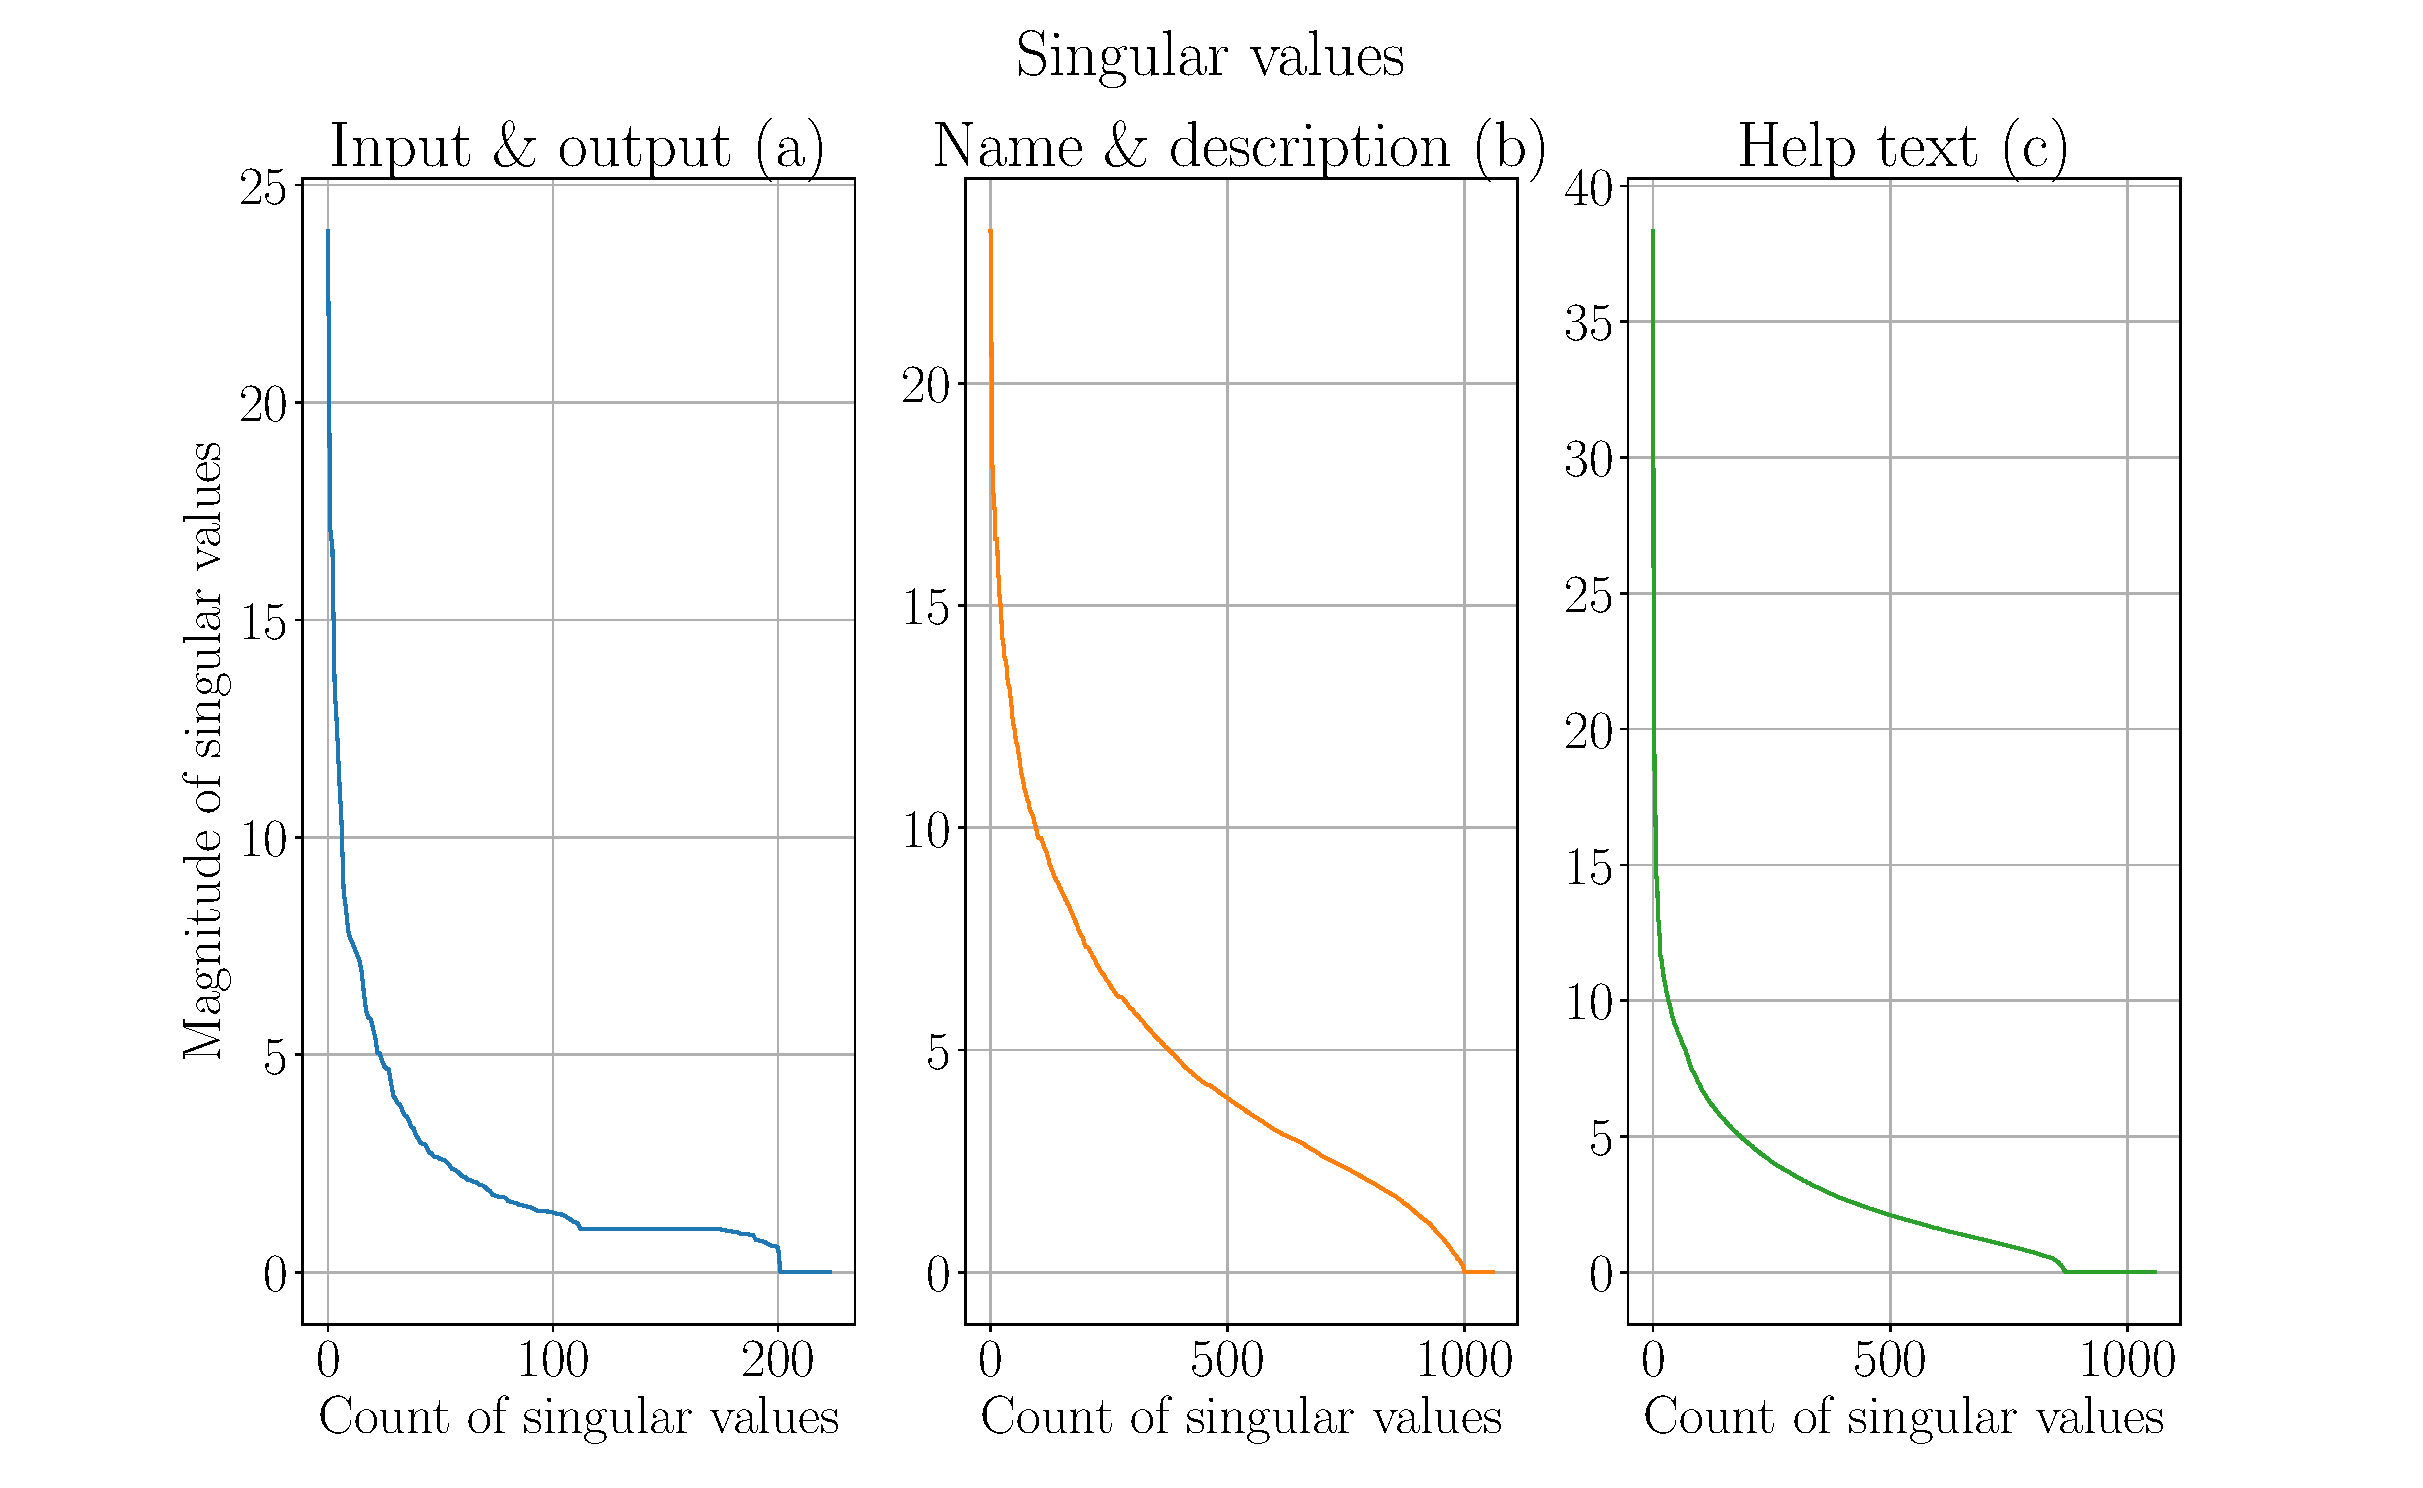
\includegraphics[scale=0.35]{figures/Singular_values.pdf}}
    \caption[Singular values of documents-tokens matrices]{\textbf{Singular values of the documents-tokens matrices}: The plot shows singular values computed using singular value decomposition (equation 5). The diagonal matrix $S$ contains these singular values sorted in descending order. We can see that in (a), (b) and (c) that very few singular values have higher mangnitude and most of the singular values are smaller.}
\end{centering}
\end{figure}

\begin{figure}[h]
\begin{centering}
    {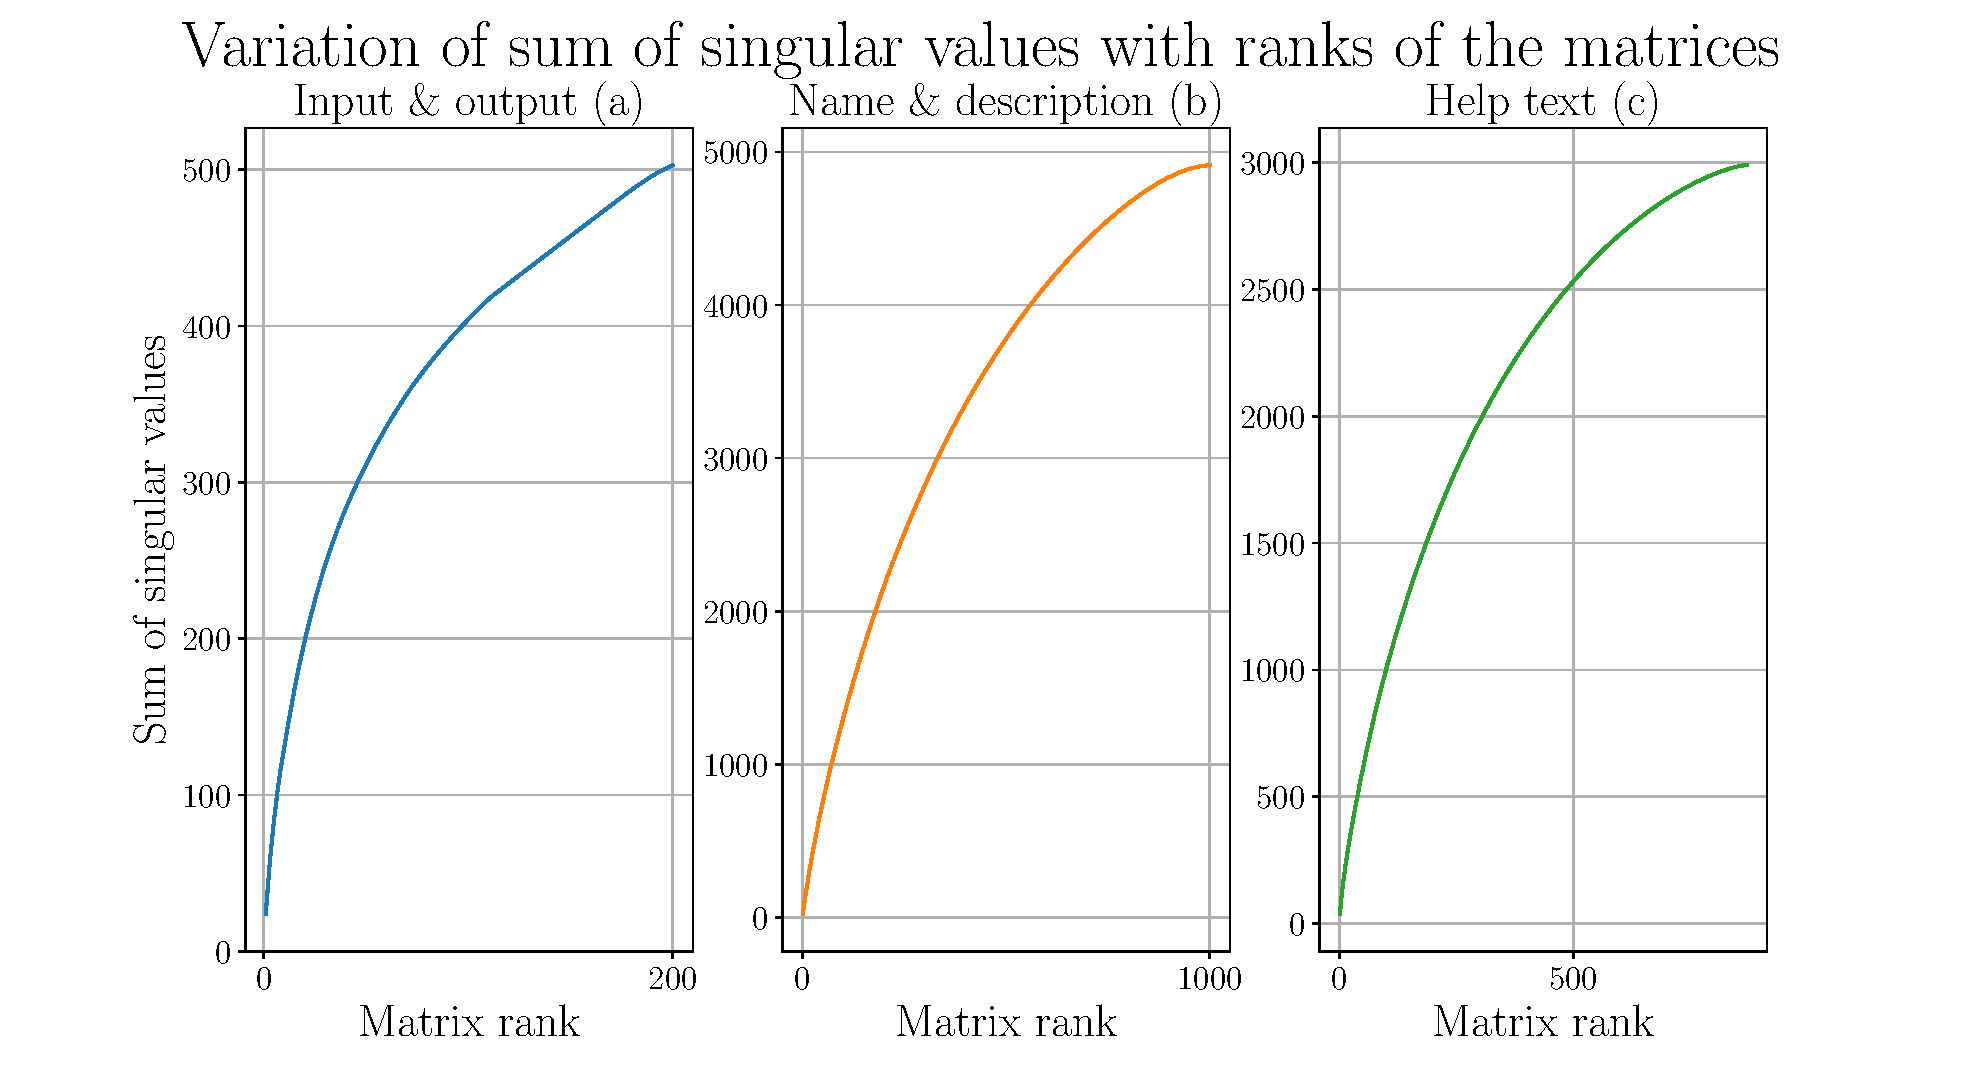
\includegraphics[scale=0.45]{figures/Sum_singular_ranks.pdf}}
    \caption[Singular values of documents-tokens matrices with their respective ranks]{\textbf{Sum of singular values with matrix rank}: The plot shows an easier way to see how the sum of singular values varies with a documents-tokens matrix rank for the three attributes. Here the (a), (b) and (c) show separately this variation as the ranks of these matrices and sum of singular values differ.}
\end{centering}
\end{figure}

\begin{figure}[h]
\begin{centering}
    {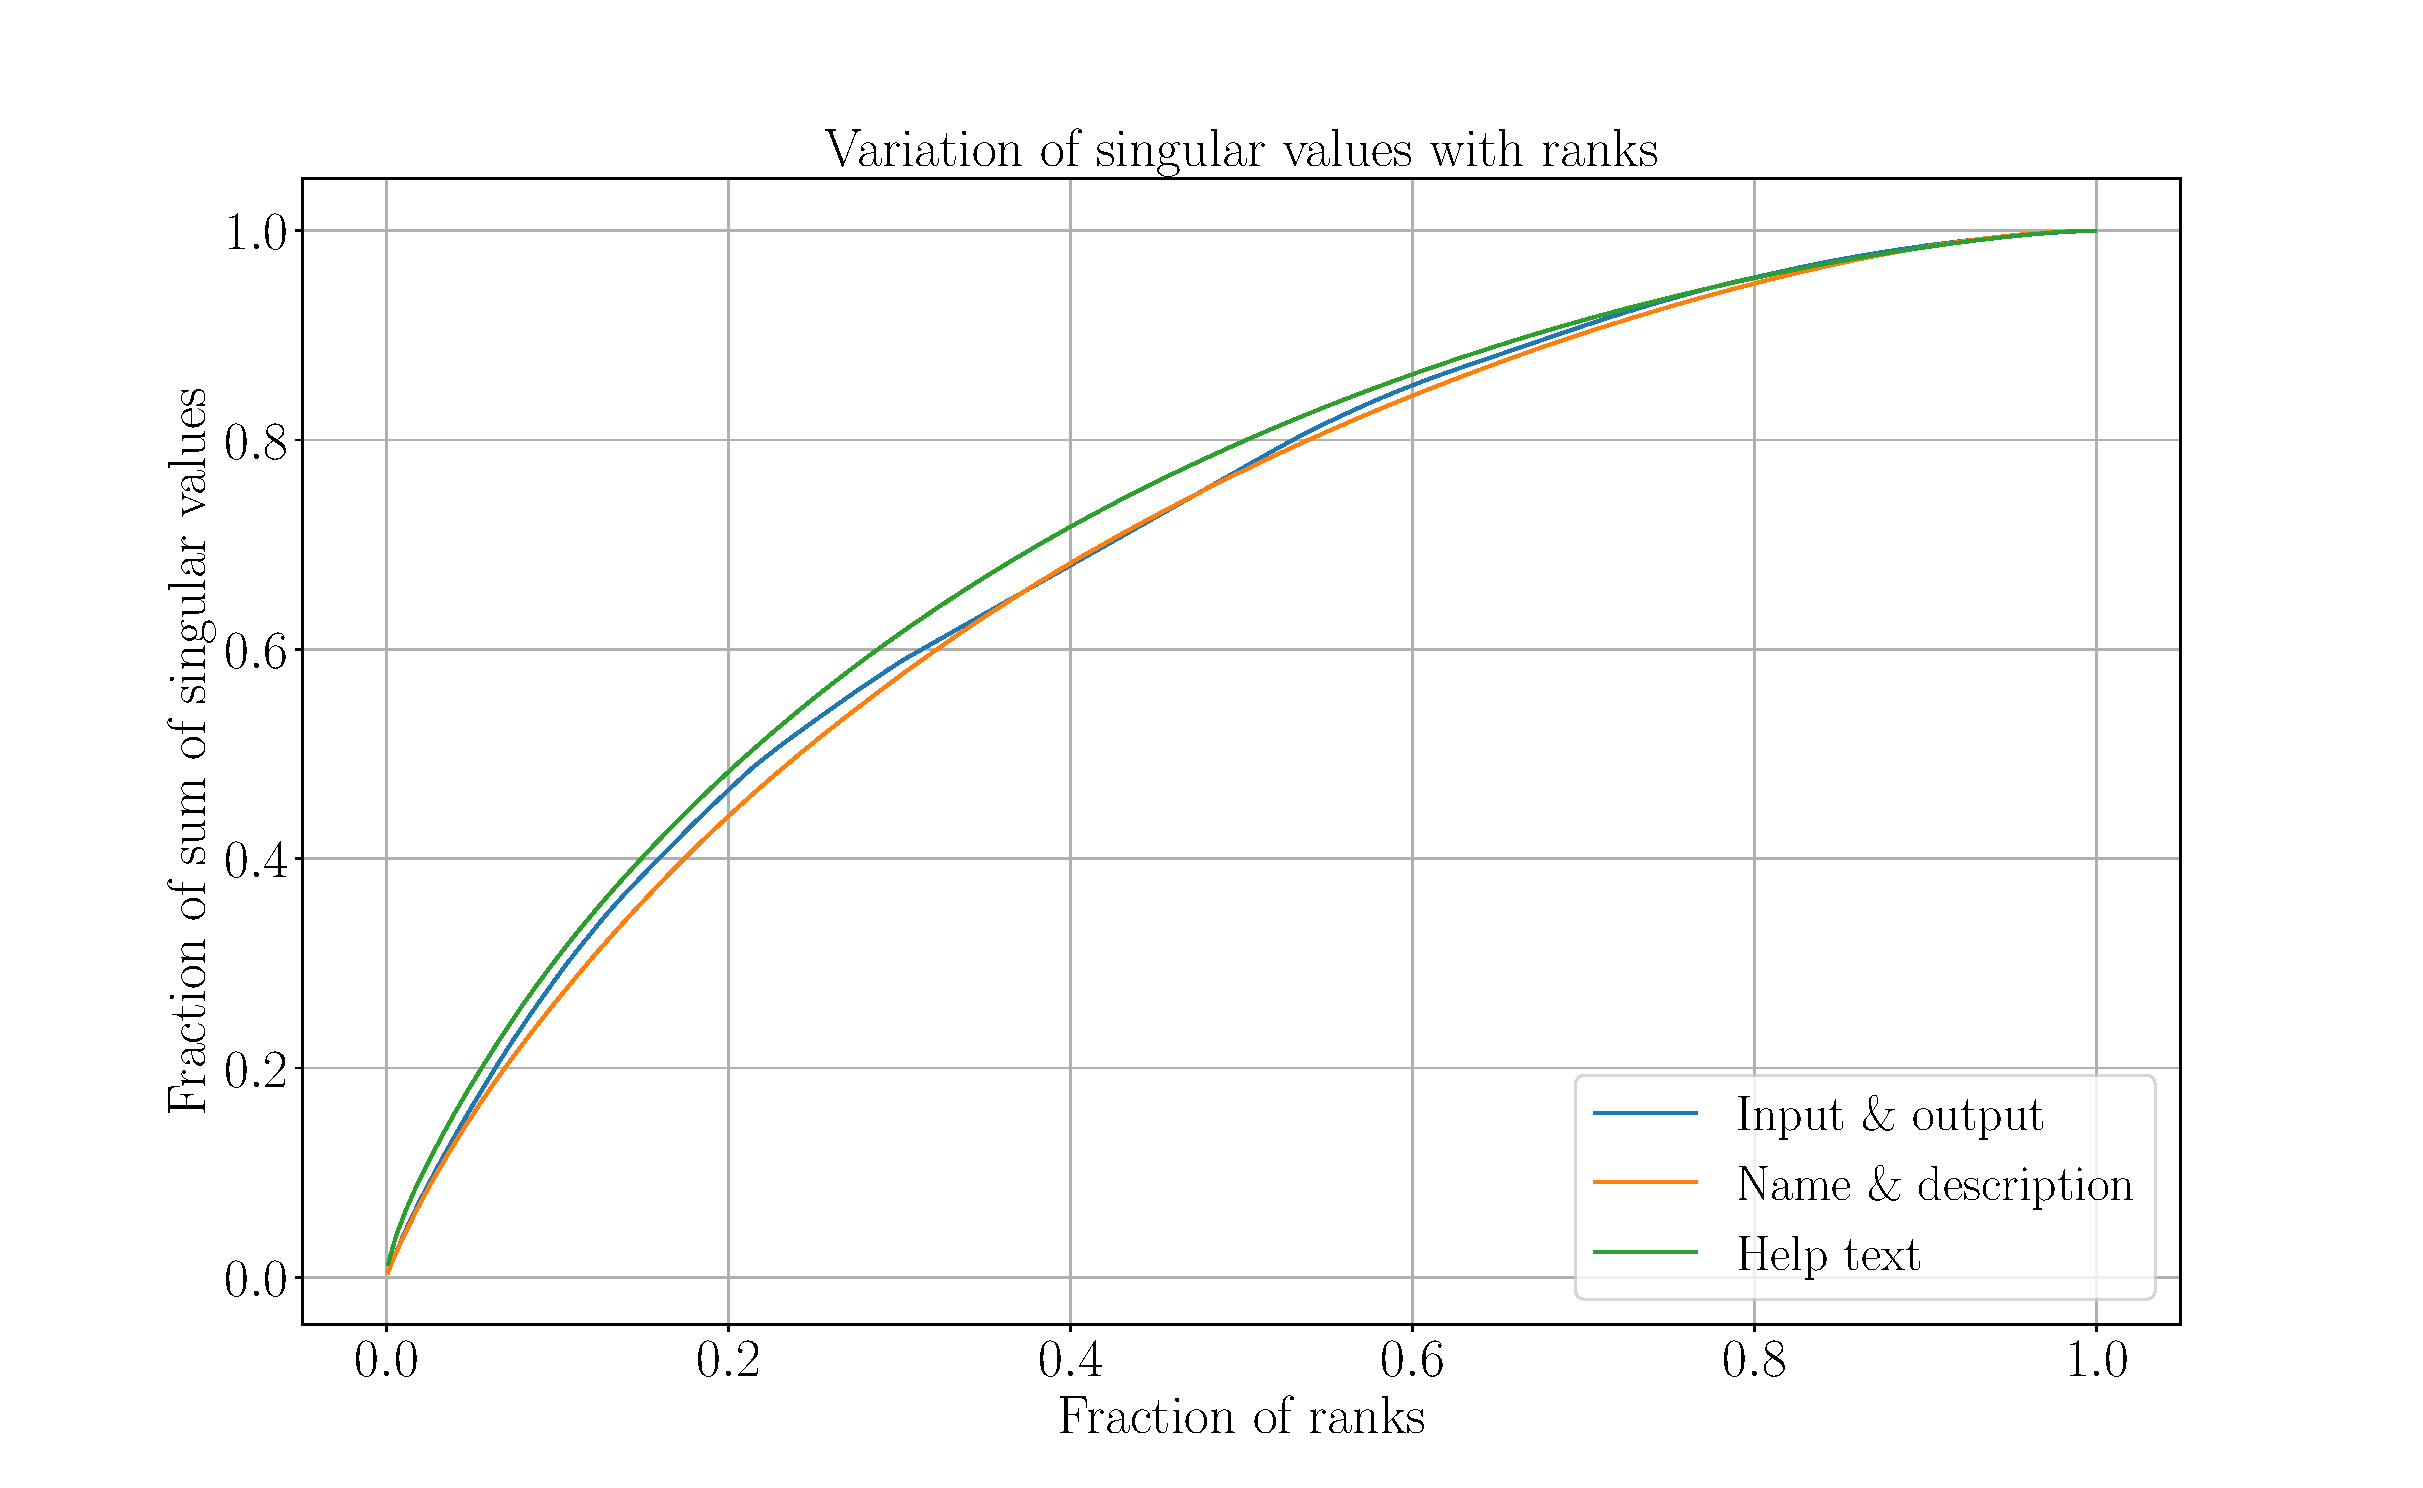
\includegraphics[scale=0.4]{figures/Fraction_ranks_singular_values.pdf}}
    \caption[The variation of fraction of ranks of documents-tokens matrices with the fraction of sum of singular values]{\textbf{The variation of fraction of ranks of documents-tokens matrices with the fraction of sum of singular values}: This plot merges the results of the figure 10 into one plot. As the ranks of document-term matrices and sum of singular values vary, we convert them to respective percentages. $rank_{fraction} = \frac{k}{N}$ where $k$ is the reduced rank and $N$ is the full-rank of a matrix For example $0.2$ on the rank axis (x-axis) means $20\%$ of the original rank of a matrix. Similarly, y-axis shows the fraction of the sum of all singular values $ sum_{fraction} = \frac{\sum_{i=1}^k}{\sum_{i=1}^K}$ where $K$ is the number of all singular values.}
\end{centering}
\end{figure}

We reduce the rank of the original documents-tokens matrices and compute the dense and low-rank approximations. Figure 12 shows the low-rank matrices for name and description and help text attributes. To compute this, we use only $5\%$ of the full-rank. We can compare it with figure 7 and verify that it is more dense than figure 7. In these low-rank matrices, we get dense vector representations for documents along the rows. In each matrix, each row contains a vector for one document. Using these documents vectors, we can compute the correlation or similarity using a similarity measure. There are multiple similarity measures which can be used like euclidean distance, cosine similarity, manhattan distance, jaccard index and many more. In our case, we use cosine angle similarity for name and description and help text and jaccard index for input and output file types to compute the correlation between vectors. We get a positive real number between $0.0$ and $1.0$ as similarity score between a pair of vectors specifying how similar they are. The higher the score, higher is the similarity. Computing this similarity for all the documents gives us a similarity matrix $S_{n \times n}$ where $n$ is the number of documents (tools). This square, symmetric matrix is called as similarity or correlation matrix. We compute three such matrices, each corresponding to one attribute (input and output file types, name and description and help text).
  
\begin{figure}[h]
\begin{centering}
    {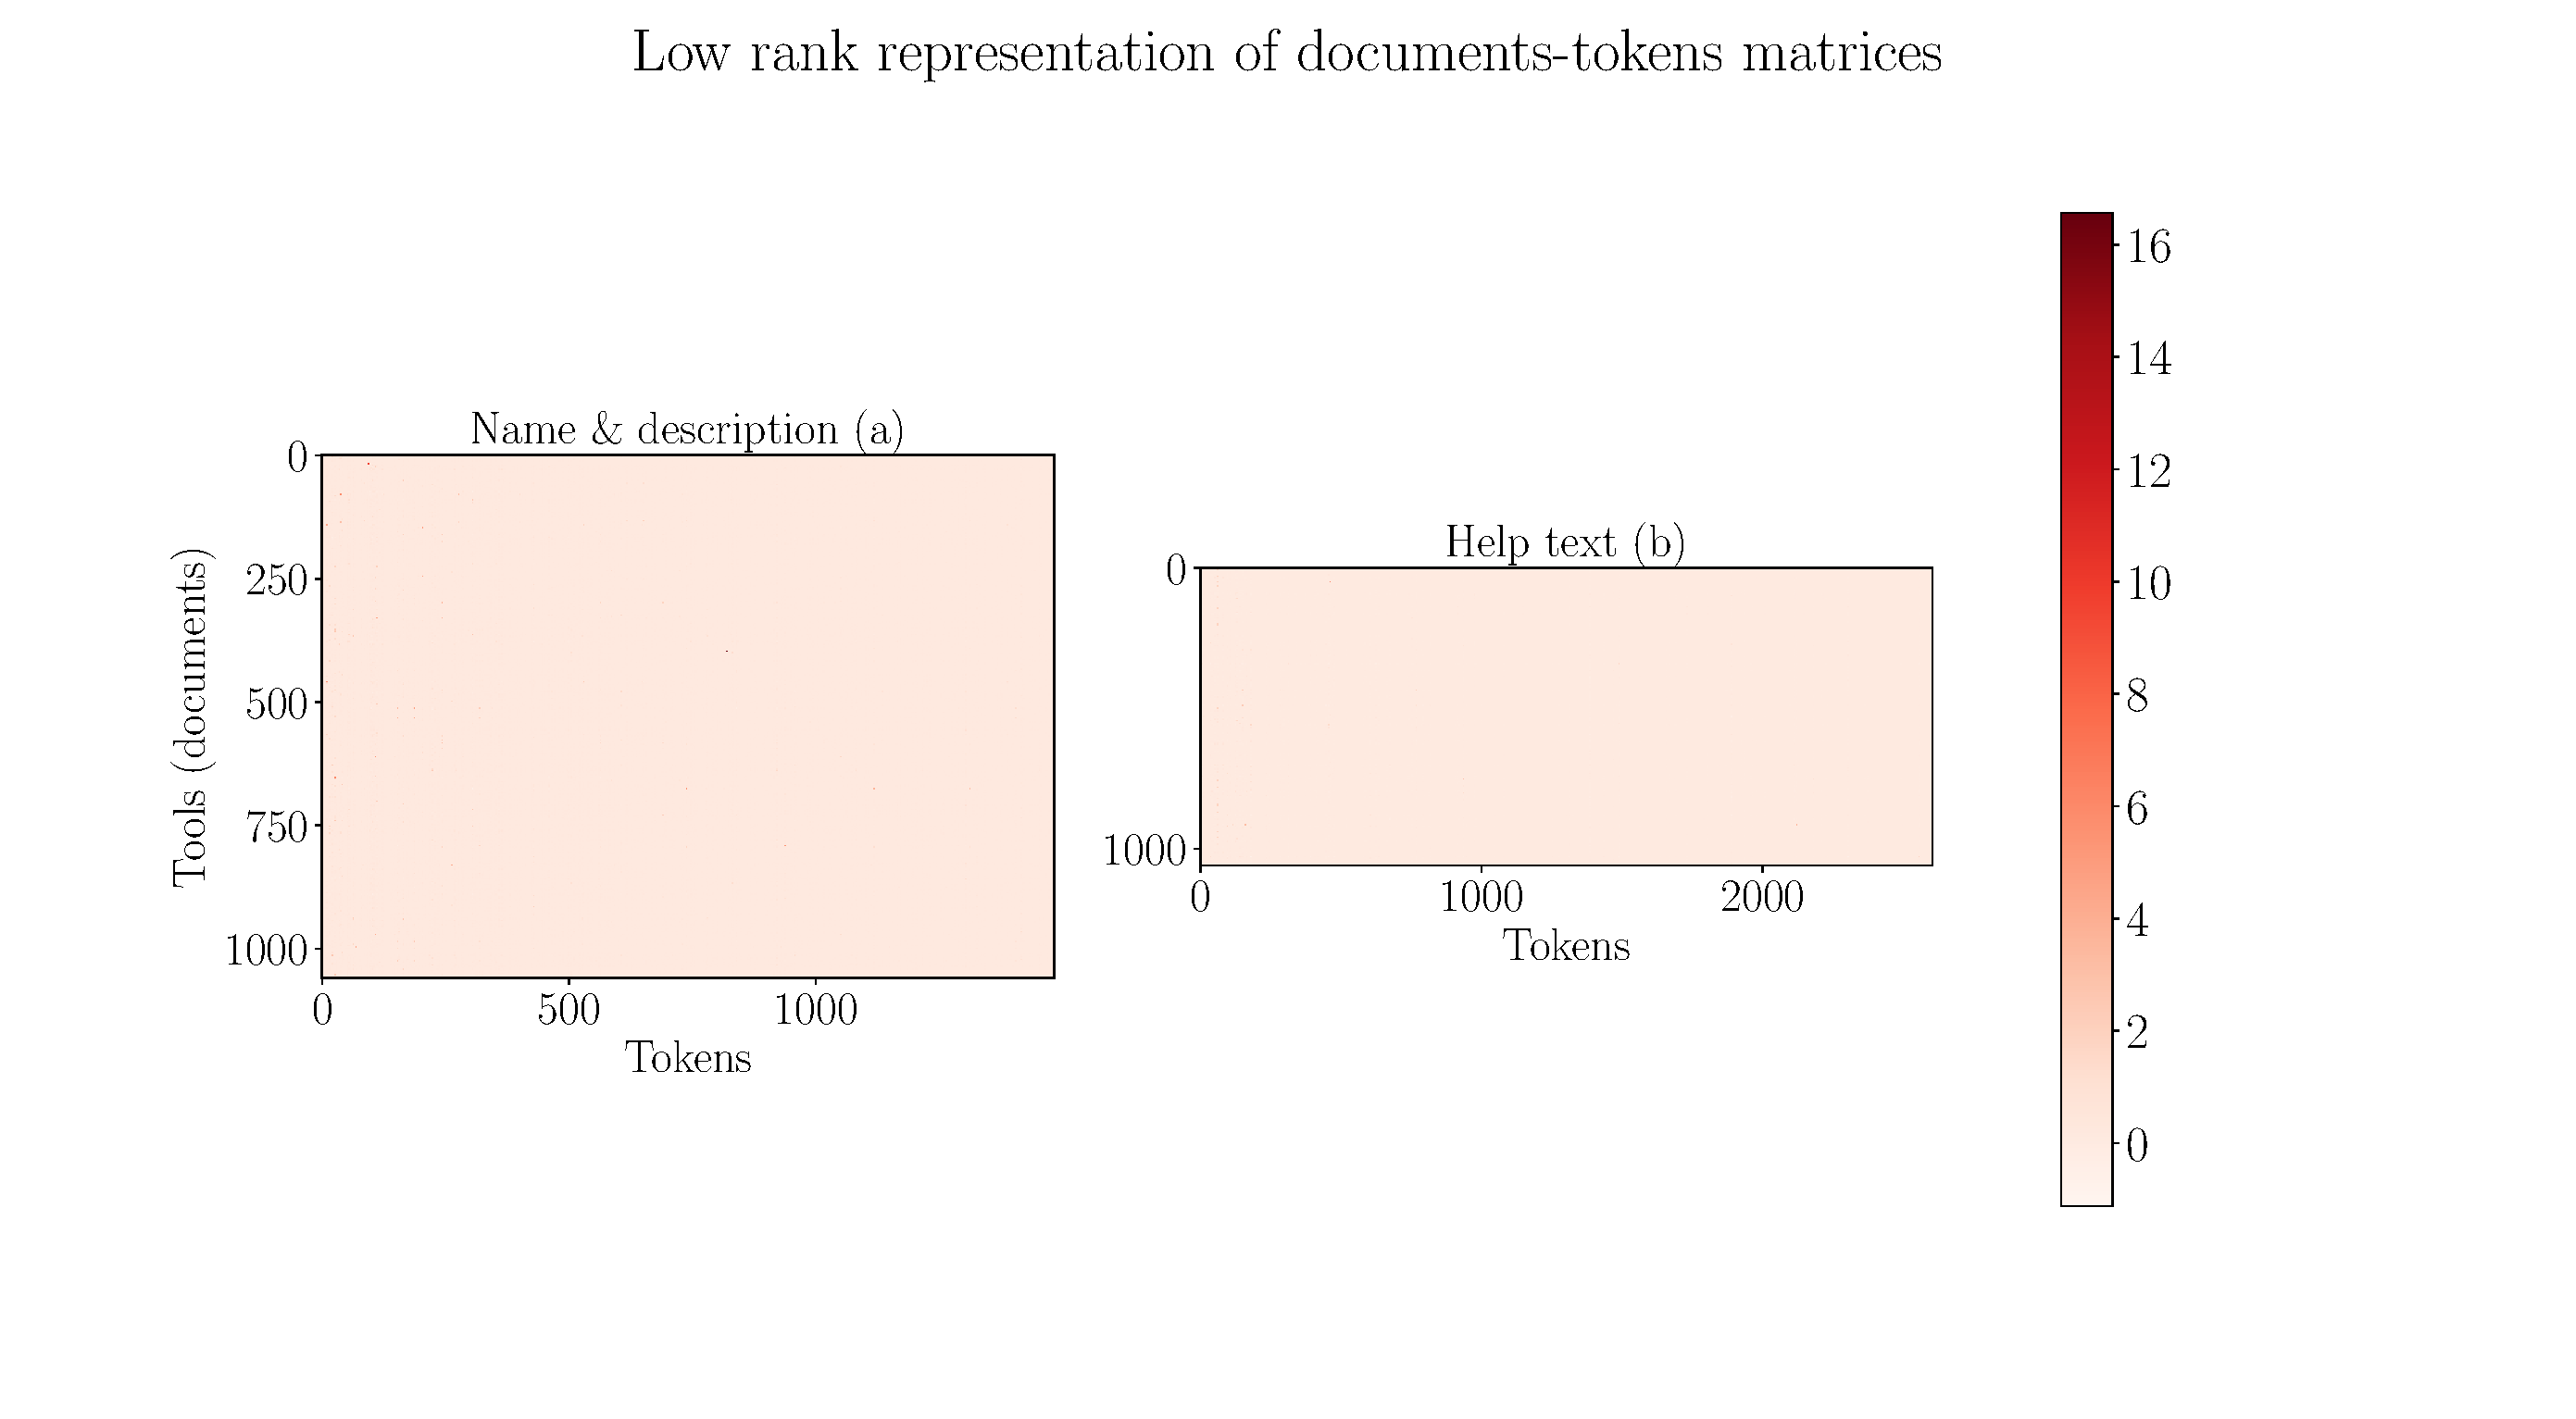
\includegraphics[scale=0.35]{figures/Document_tokens_low_rank.pdf}}
    \caption[Low-rank representations of documents-tokens matrices]{\textbf{Low-rank representations of documents-tokens matrices}: The heatmap shows the low-rank ($5\%$ of full-rank) representations of documents-tokens matrices for name and description and help text. These matrices are more dense compared to figure 7 which shows these matrices corresponding to the full-rank representations.}
\end{centering}
\end{figure}

\subsection{Paragraph vectors}
Using latent semantic indexing (LSI), we learned dense vectors to represent each document. It learns better vector representations for documents compared to using full-rank documents-tokens matrices. One main limitation is to assess the quantity by which we need to lower the rank of a matrix in order to find the optimal results. There are ways to find the optimal reduced rank by optimizing the Frobenius norm but it is not simple. We would see in the analysis section that the similar tools for a tool are more dominated by the scores shared by the input and output file types. Due to this issue, the tools which are similar in their functions do not get pushed up in the ranking ladder. To avoid these limitations, we use an approach known as $doc2vec$ (document to vector) \cite{DBLP:journals/corr/LeM14}. It learns a dense, fixed-size vectors for each document using neural networks. These vectors are unique in a way that captures the semantics present in the documents. The documents which share similar context are represented by similar vectors. When we compute cosine distance between these vectors sharing similar context, we get a higher number (closer to 1.0). It allows the documents to have variable lengths.


\subsubsection{Approach}
Paragraph vectors approach learns vector representations for all the words present in a set of documents. The words which are used in a similar context have similar vectors. For example, words like "data" and "dataset" which are used, in general, in similar contexts have are represented by vectors that are close. The vector representations of words in a document are learnt by maximizing the following equation:

\begin{equation}
\frac{1}{T} \cdot \sum_{t=k}^{T-k} \log p(w_t|w_{t-k,...,t+k})
\end{equation}

where $T$ is the total number of words in a document, $k$ is the window size. We take a few words which make a context and using this context we try to predict each word. The probability $p$ is computed using a softmax classifier and backpropagation is used to compute the gradient and the vectors are optimized using stochastic gradient descent. To learn paragraph vectors, in addition to using words vectors, paragraph vectors are also used to learn the probability of the next words in a context. The paragraph and word vectors are averaged or concatenated to make a classifier which predicts next words in a context. There are two ways how to choose a context.

\begin{itemize}
\item Distributed memory: In this approach of learning paragraph vectors, fixed length window of words are chosen and paragraph and word vectors are used to predict the words in this context. The words vectors are shared across all the paragraphs (documents) and paragraph vector is unique to each paragraph.

\begin{figure}[h]
\begin{centering}
    {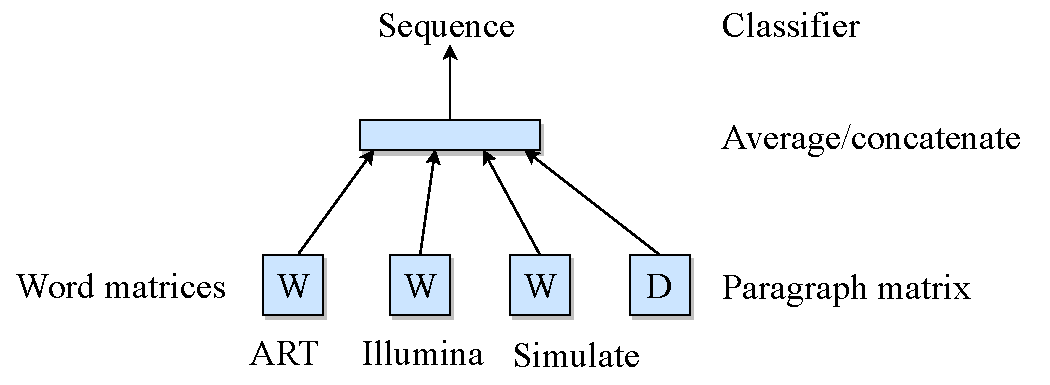
\includegraphics[scale=0.7]{figures/dm_pv.pdf}}
    \caption[Distributed memory approach for paragraph vectors]{\textbf{Distributed memory approach for paragraph vectors}: This image shows a mechanism for learning paragraph (document) vectors. $W$ is a word matrix where each word is represented by a vector. $D$ is a paragraph matrix where each paragraph (document) is represented by a vector. The word vectors are shared across all paragraphs (documents) but not the paragraph vectors. The three words "Art", "Illumina" and "Simulate" represent a context. The average or concatenated words and paragraph vectors are used to predict the "Sequence" word.}
\end{centering}
\end{figure}

\item Distributed bag of words: In this approach, words are randomly extracted from the paragraphs and from this set of words, a word is chosen randomly and predicted using the paragraph vectors. No order is followed in choosing words.
\end{itemize}

\begin{figure}[h]
\begin{centering}
    {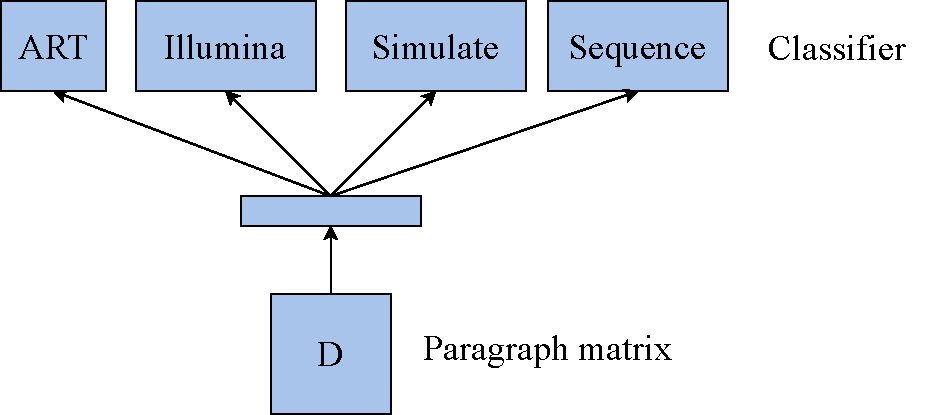
\includegraphics[scale=0.7]{figures/dbow_pv.pdf}}
    \caption[Distributed bag-of-words approach for paragraph vectors]{\textbf{Distributed bag-of-words approach for paragraph vectors}: This image shows how only paragraph vectors are learned by predicting a random word chosen from a randomly selected set of words. In this approach, the order of the words does not matter.}
\end{centering}
\end{figure}

The figures 13 and 14 are inspired from the original work - 
Distributed Representations of Sentences and Document\footnote{\label{pv}\url{https://arxiv.org/abs/1405.4053}}. The second form of learning paragraph vectors is simple and we use it to learn documents (paragraphs) vectors for name and description and help text attributes. We learn only the paragraph vectors which makes it less computationally expensive \cite{DBLP:journals/corr/LeM14} as the number of parameters is less compared to the distributed memory model which learns word vectors as well. The number of parameters in distributed bag-of-words is $\approx N \times z$ where $N$ is the number of paragraphs (documents) and $z$ is the dimensionality of each vector.

\section{Similarity measures}
From latent semantic analysis and paragraph vectors approaches, we generate vectors for the documents that belong to the three attributes. To find similarity between a pair of vectors, we can apply some similarity measures to get a similarity score. This score quantifies how much similar a pair of documents are. In this work, we use two similarity measures - cosine similarity and jaccard index. Both of these measures return a positive real number between $0$ and $1$ as a similarity score.

\subsection{Cosine similarity}
It calculates the cosine angle value between a pair of document vectors. Let's say we have two vectors, $x$ and $y$. We can write:
\begin{equation}
x \cdot y = |x| \cdot |y| \cdot \cos{\theta}
\end{equation}

\begin{equation}
\cos{\theta} = \frac {x \cdot y}{|x| \cdot |y|} 
\end{equation}

where $|x|$ is the norm of the vector $x$. If the norm is $0$, we use $0$ for the value of $\cos{\theta}$. $x \cdot y$ is the dot product of vectors $x$ and $y$. The values emitted by this similarity follows a natural progression that if the documents are dissimilar, then it is $0$ and if completely similar, it is $1.0$. Otherwise it lies between $0.0$ and $1.0$. This score can also be understood as a kind of probability of similarity between a pair of documents\footnote{\url{https://nlp.stanford.edu/IR-book/html/htmledition/dot-products-1.html}}.


\subsection{Jaccard index}
Jaccard index is a measure of similarity between two sets of entities and is given by the equation:

\begin{equation}
j = \frac{A \cap B}{A \cup B}
\end{equation}
where $A$ and $B$ are two sets. $\cap$ is the number of entities present in both the sets and $\cup$ is the sum of unique entities present in sets $A$ and $B$ \cite{Ivchenko1998}. We use this measure to compute the similarity between two tools based on their file types. For example, "LinearRegression" has 3 file types: $tabular$, $input$ and $pdf$. Another tool "LDAAnalysis" has $tabular$ and $txt$ as file types. The jaccard index for this pair of tools would be:

\begin{equation}
j = \frac{Length[(tabular, input, pdf) \cap (tabular, txt)]}{Length[(tabular, input, pdf) \cup (tabular, txt)]} = \frac{1}{4} = 0.25
\end{equation}

\section{Optimization}
We get similarity matrices after applying similarity measures on the document vectors, one each for input and output file types, name and description and help text attributes. These matrices have the same dimensions ($N \times N$, $N$ is the number of documents (tools)). To combine these matrices, one simple idea would be to take an average of the corresponding rows of similarity scores from the matrices. Doing this, we get combined similarity scores of one document (tool) with all other documents (tools). Iterating this process for all the documents would give us a similarity matrix which contains similarity scores of documents with all the other documents. The diagonal entries of this matrix would be $1.0$ and all the other entries would be a positive real number between $0.0$ and $1.0$. Another way to find the combination is to learn the weights on the rows from three matrices and then combine them to obtain optimal similarity scores for a document (tool). The weights are positive real numbers between $0.0$ and $1.0$ and for each row, they sum up to $1.0$. Instead of using fixed importance factors (weights) of $1/3$ ($3$ is the number of matrices), we use an optimization technique to find these real numbers and then combine the matrices by multiplying with these weights to obtain a weighted average optimal similarity matrix.

\begin{equation}
S_k^{optimal} = w^k_{io} \cdot S^k_{io} +  w^k_{nd} \cdot S^k_{nd} + w^k_{ht} \cdot S^k_{ht}
\end{equation}

where $w$ is a positive, real number and satisfy $w^k_{io} + w^k_{nd} + w^k_{ht} = 1$. 
$S^k_{io}$, $S^k_{nd}$ and $S^k_{ht}$ are the similarity scores (corresponding matrix rows) for $k^{th}$ tool corresponding to input and output file types, name and description and help text attributes respectively. Similarity scores $S$ has a dimensionality of $1 \times N$ where $N$ is the number of tools (documents). Each similarity score among a set of documents (tools) is independent of one another. We already have these similarity scores and need to learn the importance weights to compute the optimal similarity scores. We use gradient descent optimizer to learn the weights by minimizing an error function. To define an error function, we need to set true values where we intend to reach and then we compute mean squared error. If we look at the similarity measure, we see that the maximum similarity between a pair of documents can be $1.0$. Hence, the ideal similarity scores for a document with any other document can be at most $1.0$.

\begin{equation}
S_{ideal} = [ 1.0, 1.0, ...., 1.0 ]
\end{equation}
where $S_{ideal}$ is the ideal similarity scores for one document against all the other documents. $S_{ideal}$ has a dimensionality of $1 \times N$ where $N$ is the number of documents. Using the ideal score, we can compute the mean squared error we accrue for all the similarity scores from the three attributes separately. After computing the error, we can verify which attribute is closer to the ideal score and which are not. The attributes which measure lower error get higher weights and those which score higher error get lower weights. The next section elaborates how we use gradient descent to do the optimization.

\subsection{Gradient descent}
Gradient descent is a popular algorithm for optimizing an objective function with respect to its parameters. The parameters are the entities which we want to learn. In our case, these are the weights. The algorithm minimizes an error function. The error function which we define is the mean squared error:

\begin{equation}
Error^k_{io}(w_{io}) = \frac{1}{N - 1} \cdot \sum_{t=1}^{N-1} (w_{io} \cdot S^t_{io} - S_{ideal}) ^ 2
\end{equation}

\begin{equation}
Error^k_{nd}(w_{nd}) = \frac{1}{N - 1} \cdot \sum_{t=1}^{N-1} (w_{nd} \cdot S^t_{nd} - S_{ideal}) ^ 2
\end{equation}

\begin{equation}
Error^k_{ht}(w_{ht}) =  \frac{1}{N - 1} \cdot \sum_{t=1}^{N-1} (w_{ht} \cdot S^t_{ht} - S_{ideal}) ^ 2
\end{equation}

\begin{equation}
Error^k(w) =  \frac{1}{N - 1} \cdot \sum_{t=1}^{N-1} (w \cdot S^t - S_{ideal}) ^ 2
\end{equation}

\begin{equation}
\argmin_w Error^k(w) 
\end{equation}

\begin{equation}
\sum_{i=1}^{3} w_i = 1
\end{equation}

$Error$ is an error vector - $<Error_{io}, Error_{nd}, Error_{ht}$, $w$ is a weight vector - $<w_{io}, w_{nd}, w_{ht}>$ and $S$ similarity scores vector - $<S_{io}, S_{nd}, S_{ht}>$. $io$, $nd$ and $ht$ refer to input and output file types, name and description and help text for $Error$, $w$ and $S$. All these vectors are averaged over $N-1$ where $N$ is the number of documents (tools). We take $N-1$ in order to remove the concerned tool's similarity score with itself. To minimize the equation $20$ under the constraint given by equation $21$ where $0 \leq w_i \leq 1$ and $3$ is the number of attributes, we need to compute the gradient of the error function. The gradient specifies the rate of change of error with respect to the weights.

\begin{equation}
Gradient^k(w) = \frac{\partial Error^k}{\partial w} =  \frac{2}{N - 1} \cdot \sum_{t=1}^{N-1} (w \cdot S^t - S_{ideal}) \cdot S^t
\end{equation}

$Gradient$ is also a vector - $<Gradient_{io}, Gradient_{nd}, Gradient_{ht}>$. Using the gradient vector, we can update the weights. For this, we need to set the learning rate. Finding the right learning rate is important because a higher value can diverge the gradient descent and a lower value can slow down the learning and it could take a lot of time to converge to the minimum of the error function. For each iteration of gradient descent, we employ time-based decay of learning rate.

\begin{equation}
w^k = w^k - \eta \cdot {Gradient(w^k)}
\end{equation}
where $\eta$ is the learning rate.

\subsection{Learning rate decay}
Finding good learning rates forms an important part of the gradient descent optimization. If the learning rate is high, it poses a risk of optimizer divergence. On the other hand, if it is small, the optimizer can take a long time to converge. Both these situations are underisable. But, we can avoid these drawbacks by starting out with a small learning rate and gradually decrease it over the iterations. It is called as a time-based decay of the learning rate \cite{articleRuderS}.

\begin{equation}
lr^{t+1} = \frac{lr^t}{( 1 + ( decay * iteration ) )}
\end{equation}
where $lr^{t+1}$ and $lr^t$ are the learning rates for $t+1$ and $t$ iterations, $decay$ controls how steep or flat the learning rate curve is and $iteration$ is the gradient descent iteration number. A higher value of decay makes the learning rate curve steep as the learning rate drops quickly. A lower value can make the curve flat which can slow down the learning.

\begin{figure}[h]
\begin{centering}
    {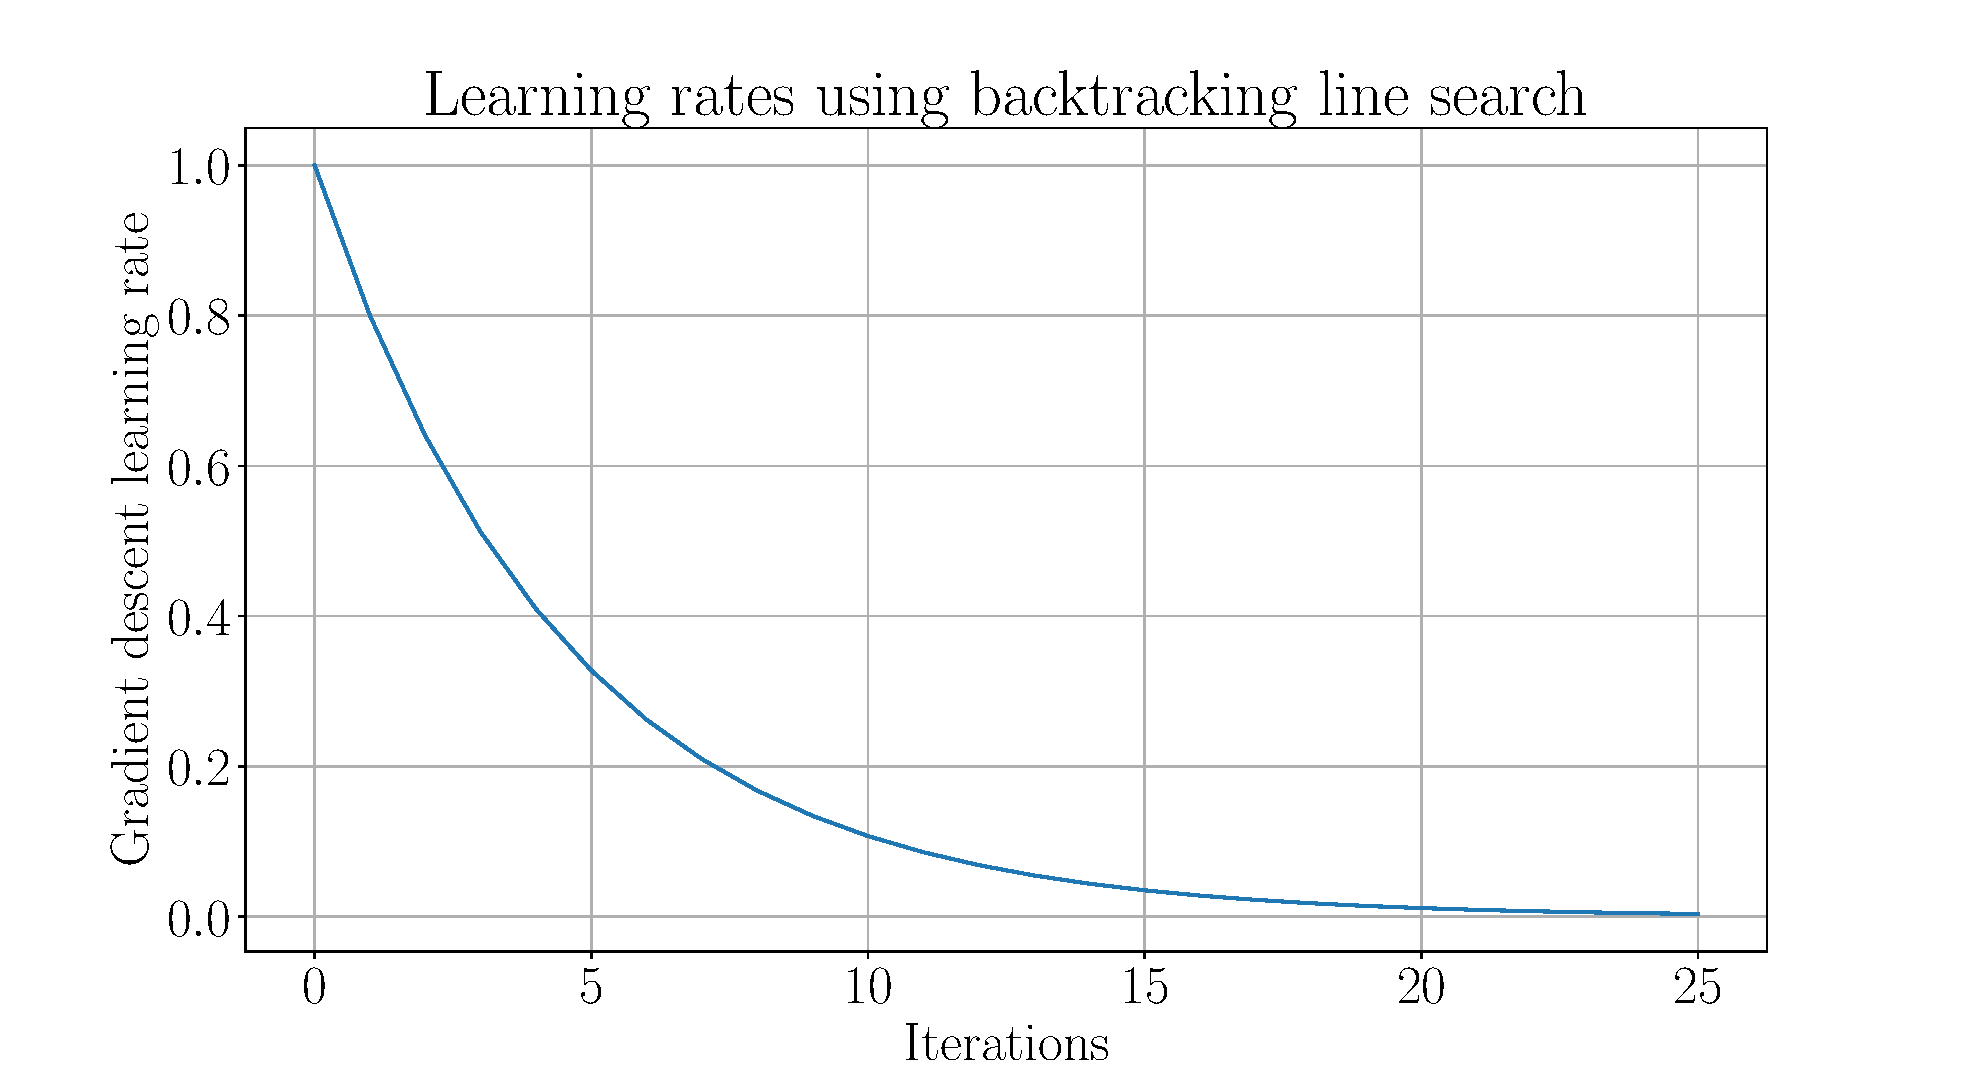
\includegraphics[scale=0.35]{figures/Learning_rates.pdf}}
    \caption[Decay of learning rate for gradient descent optimizer]{\textbf{Decay of learning rate for gradient descent optimizer}: The plot shows how the learning rate for gradient descent evolves with iterations. It starts with a small value and decreases gradually over time. It is essential to have learning rates which neither drops too quickly or too slowly. Both of these ways can lead to divergence or slow convergence of the optimizer.}
\end{centering}
\end{figure}

\subsection{Weight update}
\subsubsection{Momentum}
To reach the minimum point of our convex error function (equation 20), we need to go down continuously without being blocked at the saddle points. These saddle points are where the derivative of a function is zero. Adding a momentum term to the weight parameter, we expect to avoid the local minima and should be able to converge to the lowest point quickly. It gives the necessary push to keep going down the convex error function by adding a fraction of the previous step update to the current update \cite{articleRuderS, Sutskever}. We compute the weight parameter update for each iterations using:

\begin{equation}
update_{t+1} = \gamma \cdot update_{t} - \eta \cdot Gradient(w^t)
\end{equation}

\begin{equation}
w_{t+1} = w_t + update_{t+1}
\end{equation}

where $update_{t+1}$ is the update for changing the weight parameter for the current iteration $t+1$. $update_{t}$ is the previous iteration update. $\eta$ is the learning rate and $Gradient$ is with respect to the weight parameter $w_t$. 

\subsubsection{Nesterov’s accelerated gradient}
The inclusion of momentum is useful to get necessary advance towards finding the minimum of the error function. However, the speed of going down the slope of the error function should become less if there is a possibility of change in gradient direction. In this situation, the speeding up can be avoided by estimating the forthcoming gradient (gradient for the next step) and then correcting it \cite{Botev}. We update the weight parameter using the following equations:

\begin{equation}
update_{t+1} = \gamma \cdot update_t - \eta \cdot Gradient(w_t + \gamma \cdot update_t)
\end{equation}

\begin{equation}
w_{t+1} = w_t + update_{t+1}
\end{equation}

\subsubsection{Gradient verification}
We compute gradient using equation 21 and use it to update our weight parameters. To verify that the computed gradient is correct, we can approximate this gradient using the error function which we formulated in equation 19.

\begin{equation}
Gradient(w) = \frac{\partial Error}{\partial w} \approx \frac{Error(w + \epsilon) - Error(w - \epsilon)}{2 \cdot \epsilon} 
\end{equation}
where $\epsilon$ is a very small number ($\approx10^{-4}$). Figure 16 shows the difference of the actual and approximated gradients for all the three attributes.

\begin{figure}[h]
\begin{centering}
    {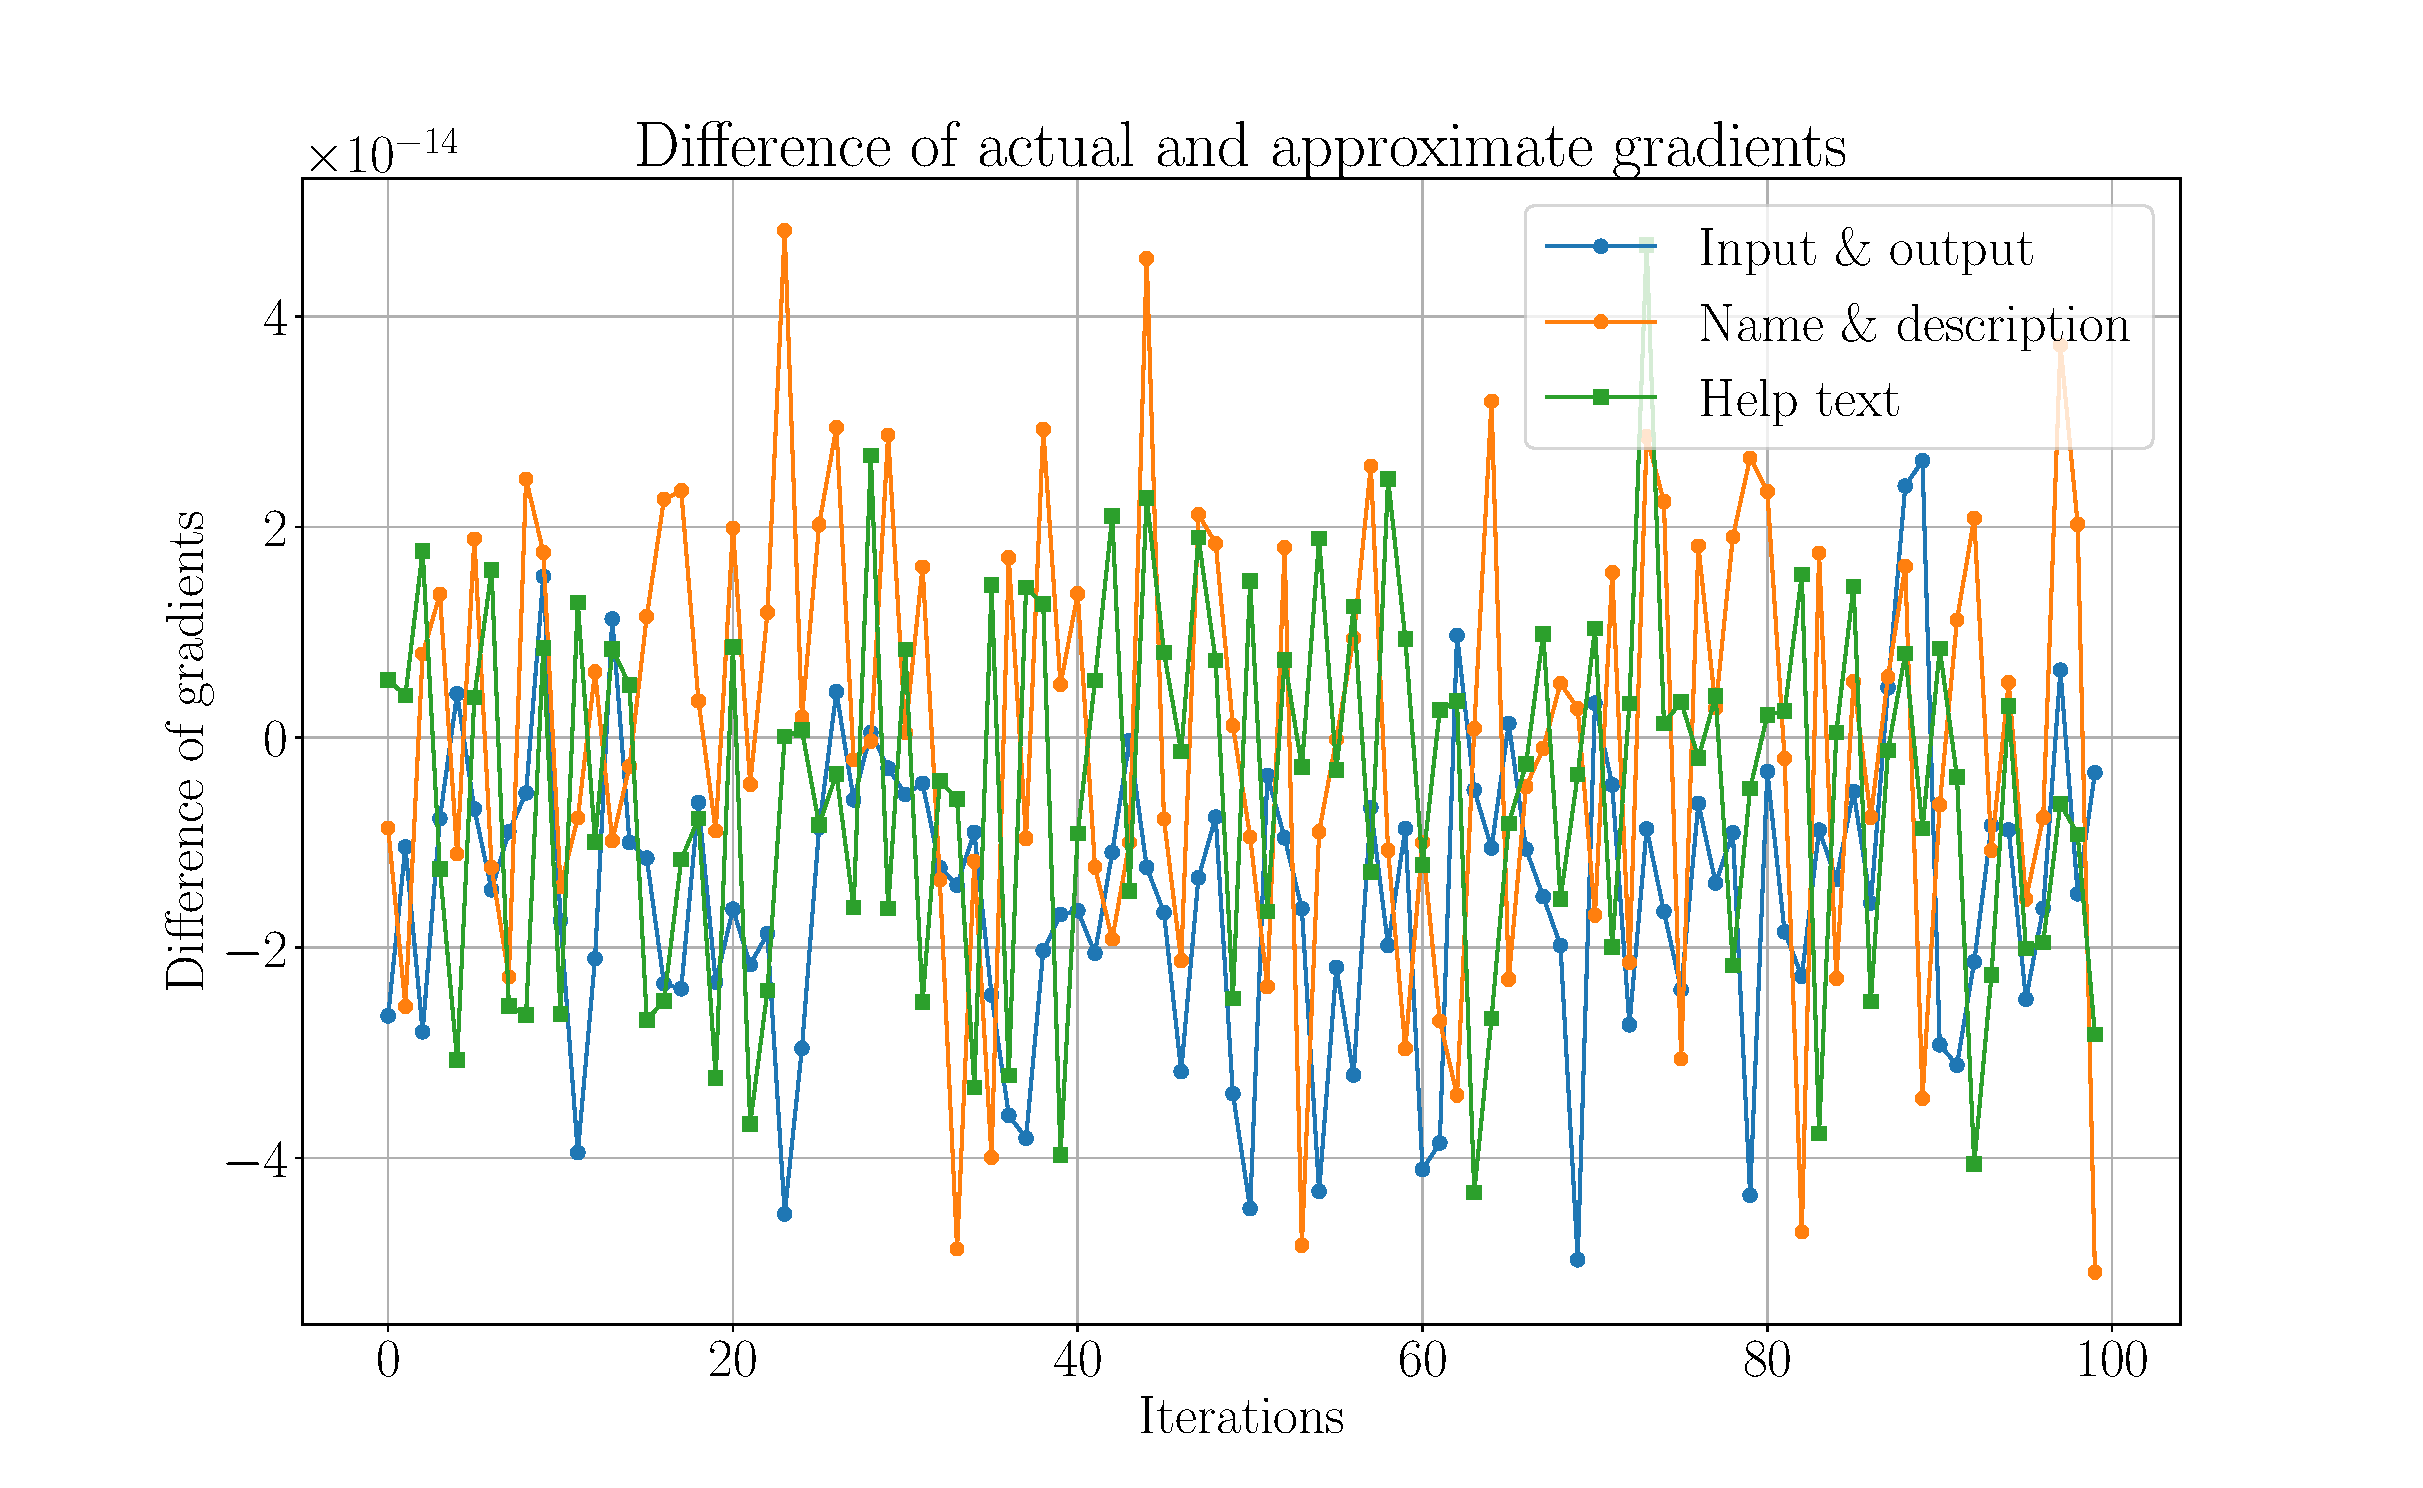
\includegraphics[scale=0.35]{figures/Difference_gradients.pdf}}
    \caption[Verification of gradient for the error function]{\textbf{Verification of gradient for the error function}: The plot checks that the difference between the actual and approximated gradients for all the attributes across all tools computed over 100 iterations is close to 0. Gradient plays an important role in learning and it should be estimated correctly. The difference of gradients is consistently $\approx 10^{-14}$ which means that the actual and approximated gradients are same and the gradient we have computed using partial derivatives is correct.}
\end{centering}
\end{figure}